%input macros (i.e. write your own macros file called MacroFile1.tex)
%\newcommand{\PdfPsText}[2]{
  \ifpdf
     #1
  \else
     #2
  \fi
}

\newcommand{\IncludeGraphicsH}[3]{
  \PdfPsText{\includegraphics[height=#2]{#1}}{\includegraphics[bb = #3, height=#2]{#1}}
}

\newcommand{\IncludeGraphicsW}[3]{
  \PdfPsText{\includegraphics[width=#2]{#1}}{\includegraphics[bb = #3, width=#2]{#1}}
}

\newcommand{\InsertFig}[3]{
  \begin{figure}[!htbp]
    \begin{center}
      \leavevmode
      #1
      \caption{#2}
      \label{#3}
    \end{center}
  \end{figure}
}


%%% Local Variables: 
%%% mode: latex
%%% TeX-master: "~/Documents/LaTeX/CUEDThesisPSnPDF/thesis"
%%% End: 


\documentclass[oneside,12pt,pdftex]{Classes/CUEDthesisPSnPDF}


\pdfinfo { /Title (Mémoire de Master Informatique) /Creator (TeX)
  /Producer (pdfTeX) /Author (Arnaud Bletterer
  arnaud.bletterer@etu.unistra.fr) /Subject (Outils multidimensionnels
  de déformation) /Keywords (MSc, Mémoire)} \pdfcatalog { /PageMode
  (/UseOutlines) /OpenAction (fitbh) }

\title{Outils multidimensionnels \\ de déformation}

\author{\href{mailto:arnaud.bletterer@etu.unistra.fr}{Arnaud
    Bletterer}} \collegeordept{\href{http://mathinfo.unistra.fr/}{UFR de
    Mathématique-Informatique}}
\university{\href{http://www.unistra.fr}{Université de Strasbourg}}
% insert below the file name that contains the crest in-place of
% 'UnivShield'
\crest{
\includegraphics[scale=0.5, viewport=850 270 0 0]{UnivStrasbourg}}

% insert below the file name that contains the crest in-place of
% 'UnivShield' \crest{\IncludeGraphicsW{UnivShield}{40mm}{14 14 73
% 81}}
%
\renewcommand{\submittedtext}{\textbf{Mémoire soumis pour le diplôme de :}}

\direction{\textbf{Sous la direction de :} \\ 
Mme. Dominique Bechmann, Professeure, ICube\\ 
Mme. Isabelle Charpentier, Chargée de Recherche CNRS, ICube\\
M. Pierre Kraemer, Maître de conférences, ICube\\
\textbf{Rapporté par :} \\
M. Basile Sauvage, Maître de conférences, ICube}

\degree{Master mention Informatique, \\ Spécialité Informatique et
  Sciences de l'Image} \degreedate{Juin 2014}

% turn of those nasty overfull and underfull hboxes
\hbadness=10000 \hfuzz=50pt

% Put all the style files you want in the directory StyleFiles and
% usepackage like this:
\usepackage{StyleFiles/watermark}

% Comment out the next line to get single spacing

\begin{document}

% \language{english}

% A page with the abstract on including title and author etc may be
% required to be handed in separately. If this is not so, then comment
% the below 3 lines (between '\begin{abstractseparte}' and
%   'end{abstractseparate}'), normally like a declaration ... needs
%   some more work, mind as environment abstracts creates a new page!
%   \begin{abstractseparate}
%     
% Thesis Abstract -----------------------------------------------------


%\begin{abstractslong}    %uncommenting this line, gives a different abstract heading
\begin{abstracts}        %this creates the heading for the abstract page

This is where you write your abstract ...


\end{abstracts}
%\end{abstractlongs}


% ----------------------------------------------------------------------


%%% Local Variables: 
%%% mode: latex
%%% TeX-master: "../thesis"
%%% End: 

%   \end{abstractseparate}

%   Using the watermark package which is in StyleFiles/ and to remove
%   DRAFT COPY ONLY appearing on the top of all pages comment out
%   below line \watermark{DRAFT COPY ONLY}

\maketitle

\onehalfspacing

% set the number of sectioning levels that get number and appear in
% the contents
\setcounter{secnumdepth}{3} \setcounter{tocdepth}{3}

\frontmatter % book mode only
% \pagenumbering{roman}
%% Thesis Dedictation ---------------------------------------------------

\begin{dedication} %this creates the heading for the dedication page

I would like to dedicate this thesis to my loving parents ...

\end{dedication}

% ----------------------------------------------------------------------

%%% Local Variables: 
%%% mode: latex
%%% TeX-master: "../thesis"
%%% End: 

% Thesis Acknowledgements ------------------------------------------------


%\begin{acknowledgementslong} %uncommenting this line, gives a different acknowledgements heading
\begin{acknowledgements}      %this creates the heading for the acknowlegments


And I would like to acknowledge ...


\end{acknowledgements}
%\end{acknowledgmentslong}

% ------------------------------------------------------------------------

%%% Local Variables: 
%%% mode: latex
%%% TeX-master: "../thesis"
%%% End: 

% 
% Thesis Abstract -----------------------------------------------------


%\begin{abstractslong}    %uncommenting this line, gives a different abstract heading
\begin{abstracts}        %this creates the heading for the abstract page

This is where you write your abstract ...


\end{abstracts}
%\end{abstractlongs}


% ----------------------------------------------------------------------


%%% Local Variables: 
%%% mode: latex
%%% TeX-master: "../thesis"
%%% End: 


\tableofcontents
\listoffigures

\mainmatter % book mode only
%%% Thesis Introduction --------------------------------------------------
\chapter{Introduction}

\graphicspath{ {Introduction/IntroductionFigs/PNG/}
  {Introduction/IntroductionFigs/PDF/}
  {Introduction/IntroductionFigs/} }

La modélisation géométrique a permis, dans un premier temps, de
représenter des modèles virtuels. Mais le besoin d'éditer ces modèles
a amené la modélisation géométrique a évoluer et à instaurer des
outils permettant de modifier ces modèles. Ainsi sont nés les outils
de \textit{déformation}. Dans le cadre de notre travail, nous ne nous
sommes uniquement intéressés aux déformations dites
\textit{spatiales}.
\\

La déformation spatiale consiste à déformer un objet en modifiant son
espace ambiant.  On notera \cite{Bar84} et \cite{SP86} comme étant les
premiers à avoir introduit ce type de déformation. Ce procédé a un
avantage considérable, la modification de l'espace. En effet comme la
déformation est réalisée sur chaque point de l'espace de façon
indépendante, elle n'est pas liée à la représentation interne de
l'objet. Cette propriété est essentielle, car elle permet d'assurer
que, peu importe la topologie existante entre les points de l'espace à
déformer, une même déformation de l'outil déformera l'espace de la
même manière.
\\

La première partie de ce travail consiste en la réalisation d'un
mélange de multiples outils de déformation, en s'inspirant des travaux
de \cite{JBPS11} et \cite{GPCP13}. En parallèle, une étude est faite
sur les outils de déformation de différentes dimensions, basée sur
\cite{GB08}, pour déterminer le meilleur outil associé à chaque
dimension (point, courbe, surface, volume). La dernière partie se
concentre plus particulièrement sur les modèles virtuels. Il s'agit de
fournir une génération automatique d'un outil multidimensionnel de
déformation associé à un modèle, en segmentant ce dernier et en
associant à chacune de ses segmentations l'outil de déformation le
plus adapté à sa forme.
\\

Beaucoup de méthodes existent pour déformer des points de l'espace,
mais ont des caractéristiques différentes les unes des autres. Que ce
soit au niveau de la complexité au temps d'association des points de
l'espace à l'outil, de la forme de la déformation engendrée par la
modification de l'outil, ou encore de l'élégance et de la simplicité
du modèle mathématique sous-jacent. Il n'existe aujourd'hui aucune
technique permettant de combiner les forces de chacune de ces méthodes
et de pouvoir en changer de façon interactive.
\\

Tout au long de ce travail, nos choix ont été motivés par la volonté
de fournir un outil permettant de déformer des points de l'espace de
manière interactive et fluide, et d'obtenir des formulations
mathématiques simples et claires. Le but de ce travail est de pouvoir
permettre à un utilisateur d'obtenir un outil de déformation
s'adaptant à ses besoins, en générant de façon automatique un outil
multidimensionnel de déformation, tout en lui laissant la possibilité
de paramétrer le comportement des différents outils utilisés.
%%% ----------------------------------------------------------------------


%%% Local Variables: 
%%% mode: latex
%%% TeX-master: "../thesis"
%%% End: 


% \pagebreak[4]
% \hspace*{1cm}
% \pagebreak[4]
% \hspace*{1cm}
% \pagebreak[4]

\chapter{Outils multidimensionnels}

\graphicspath{{Chapter1/Chapter1Figs/PNG/}{Chapter1/Chapter1Figs/PDF/}{Chapter1/Chapter1Figs/}}

Ce chapitre réalise un état de l'art des différentes déformations
spatiales, d'après \cite{GB08}, tout en les comparant, dans chaque
dimension, selon des critères de souplesse, facilité d'utilisation,
efficacité (en complexité) et exactitude. Ce classement va nous
permettre de choisir le meilleur outil associé à chaque dimension,
afin d'obtenir à la fin une sélection de 4 outils de dimensions
différentes sur lesquels nous allons nous baser pour réaliser les
mélanges.

\section{Déformation à base de volumes}

\section{Déformation à base de surfaces}
La difficulté des déformations à base de surfaces réside dans la
manière d'attacher les points de l'espace à une surface.

\begin{itemize}
\item{\textbf{Carreau paramétrique :}} \cite{JLQ96} a été le premier à
  proposer une solution, celle d'utiliser un carreau B-spline sur
  lequel sont projetés les points de l'espace, le long de la normale
  au plan du carreau, dans l'espace paramétrique du carreau. Ainsi
  pour déformer l'espace, l'utilisateur n'a plus qu'à déformer les
  points de contrôle du carreau. Les points de l'espace sont
  repositionnés grâce à leurs coordonnées paramétriques (précédemment
  calculées) et "reprojetés" le long de la normale au carreau déformé.
  % \begin{itemize}
  % \item{\textit{Création de l'outil de déformation :}} Les points de
  %   contrôle du carreau initial \( \mathcal{S}(u,v) \) sont disposés
  %   sur le plan XZ (Y=1). Ce carreau définit une région déformable
  %   délimitée par les bords du carreau (en X et en Z) et s'étendant
  %   à
  %   l'infini en Y.
  % \item{\textit{Association des points de l'espace à l'outil :}}
  %   Pour
  %   chaque point de l'espace \( X = (x,y,z) \) se situant dans la
  %   région contenue, des coordonnées paramétriques \( U = (u,v,w) \)
  %   sont obtenues par calcul de la projection \( X_p \) du point \(
  %   X
  %   \) sur le carreau le long de la normale à ce dernier. \( (u,v)
  %   \)
  %   est obtenu par méthode numérique de façon à ce que \(
  %   \mathcal{S}(u,v) = X_p \), et \( w \) correspond à la distance
  %   de
  %   \( X \) à \( X_p \). On obtient donc :
  %   \begin{equation}
  %     X = \mathcal{S}(u,v) + w \cdot \mathcal{N}(u,v)
  %   \end{equation}
  %   où \( \mathcal{N}(u,v) \) est le vecteur normal au point \(
  %   (u,v)
  %   \) sur la surface \( \mathcal{S} \).
  % \item{\textit{L'outil est modifié :}} Les points de contrôle sont
  %   déplacés aux positions choisies par l'utilisateur, formant un
  %   nouveau carreau \( \tilde{\mathcal{S}} \).
  % \item{\textit{L'espace est déformé :}} Les coordonnées
  %   paramétriques
  %   calculées pour chaque point de l'espace sont invariantes par
  %   déformation, ainsi les nouvelles positions sont obtenues en
  %   appliquant :
  %   \begin{equation}
  %     \tilde{X} = \tilde{\mathcal{S}}(u,v) + w \cdot \tilde{\mathcal{N}}(u,v)
  %   \end{equation}
  %   où \( \tilde{\mathcal{N}}(u,v) \) est le vecteur normal au point
  %   \( (u,v) \) de la surface déformée \( \tilde{X} \)
  % \end{itemize}
\item{\textbf{Surface étoilée :}} Un polyèdre de forme étoilée est un
  polyèdre contenant, en son intérieur, une région dite "étoilée". On
  définit une région étoilée d'un polygone comme étant une région
  depuis laquelle un rayon émis dans n'importe qu'elle direction
  n'intersecte le bord du polygone qu'une seule fois. Cette propriété
  est utile dans le domaine de la déformation car elle permet
  d'obtenir une unique paramétrisation en coordonnées polaires des
  points de l'espace, comme proposé par \cite{JL00}.
  % \begin{itemize}
  % \item{\textit{Création de l'outil de déformation :}} L'utilisateur
  %   définit une surface \( S \), représentant un polyèdre étoilé. il
  %   définit un centre \( O \) situé dans la partie étoilée du
  %   polyèdre. La surface peut avoir n'importe qu'elle
  %   représentation,
  %   à partir du moment ou celle-ci permet de réaliser des tests
  %   d'intersection entre un rayon et le bord de la surface.
  % \item{\textit{Association des points de l'espace à l'outil :}} Un
  %   rayon est construit, partant de \( O \) passant par un point de
  %   l'espace \( X \) et intersectant le bord de \( S \). La
  %   direction
  %   du rayon \( U \) et le ratio de distances de \( O \) à \( X \)
  %   et
  %   de \( O \) à \( P \) sont enregistrés.
  % \item{\textit{L'outil est modifié :}} Une surface de destination
  %   \(
  %   \tilde{S} \), avec un centre \( \tilde{O} \), est définie.
  % \item{\textit{L'espace est déformé :}} La déformation se fait en
  %   construisant un rayon partant de \( \tilde{O} \) avec la même
  %   direction \( U \), on peut ainsi obtenir l'intersection \(
  %   \tilde{P} \) entre le rayon et le bord de \( \tilde{S} \). Le
  %   point déformé \( \tilde{X} \) est placé à la même distance
  %   relative entre \( \tilde{O} \) et \( \tilde{P} \).
  % \end{itemize}
\item{\textbf{Maillage triangulaire :}} Une autre idée est d'utiliser
  un maillage triangulaire simple pour appliquer des déformations aux
  points de l'espace. \cite{KO03} a été le premier à utiliser ce genre
  d'outil. Il définit que les triangles du maillage contribuent à
  déformer une zone de l'espace proche en réalisant une moyenne
  pondérée, et que chacun d'entre eux influent sur une zone sphérique
  autour d'eux. L'avantage de cette technique est de permettre une
  configuration assez générale des triangles (non nécessairement
  connexes), à partir du moment où ceux-ci ne sont pas dégénérés
  (sommets distincts).
  % \begin{itemize}
  % \item{\textit{Création de l'outil de déformation :}} L'utilisateur
  %   place un certain nombre de triangles, ils n'ont pas besoin
  %   d'être
  %   connexes et peuvent s'intersecter. La seule restriction est
  %   qu'ils
  %   ne soient pas dégénérés.
  % \item{\textit{Association des points de l'espace à l'outil :}} Un
  %   système de coordonnées est associé à chaque triangle, un sommet
  %   est choisi pour être l'origine \( O_i \), les deux arêtes
  %   incidentes à ce sommet sont les axes \( U_i \) et \( V_i \) et
  %   la
  %   normale du triangle est le dernier axe, \( W_i \). On peut noter
  %   que le système de coordonnées n'est pas orthogonal, sauf dans le
  %   cas d'un triangle rectangle. On associe à chaque point de
  %   l'espace
  %   des coordonnées paramétriques \( U = (u_i,v_i,w_i) \) locales à
  %   chaque triangle ainsi qu'un poids \( k_i \), qui décroit de
  %   façon
  %   linéaire dans une sphère d'influence autour de chaque triangle,
  %   dont la taille varie en fonction de la taille du triangle.
  % \item{\textit{L'outil est modifié :}} Les triangles sont modifiés,
  %   soit en déplaçant des sommets des triangles, soit en déplaçant
  %   des
  %   points de l'espace et en recalculant la position des triangles
  %   (par reverse-engineering) pour enfin déplacer le reste des
  %   points
  %   de l'espace.
  % \item{\textit{L'espace est déformé :}} Encore une fois, les
  %   coordonnées paramétriques calculées sont invariantes par
  %   déformation, on peut donc calculer la nouvelle position des
  %   points
  %   de l'espace par rapport à chaque triangle :
  %   \begin{equation}
  %     \tilde{X}_i = \tilde{O}_i + u_i\tilde{U}_i + v_i\tilde{V}_i +
  %     w_i\tilde{W}_i
  %   \end{equation}
  %   Au final, la position d'un point de l'espace est calculée comme
  %   une combinaison linéaire des coordonnées associées à chaque
  %   triangle :
  %   \begin{equation}
  %     \tilde{X} = \sum_i \frac{k_i\tilde{X}_i}{\sum_i k_i}
  %   \end{equation}
  % \end{itemize}
\item{\textbf{Cage :}} La cage est outil le plus utilisé ces dernières années en
  terme de déformation spatiale. Un polygone de contrôle (quelconque)
  est créé et permet de définir des coordonnées paramétriques pour les
  points de l'espace par rapport aux sommets du polygone. Pour
  calculer ces coordonnées, il existe plusieurs méthodes, mais
  dérivent toutes des coordonnées barycentriques généralisées. Les
  coordonnées barycentriques généralisées sont une extension des
  coordonnés barycentriques afin de permettre de calculer des
  coordonnées non plus par rapport à un simplexe (triangle en dimension
  2), mais par rapport à n'importe quelle cellule (polygone quelconque
  en dimension 2).

  On définit les positions des points de l'espace $p$ comme étant une
  combinaison linéaire des positions des sommets du polygone de
  contrôle $v_i$.
  \begin{equation}
    p = \sum_{i=0}^n w_iv_i
  \end{equation}
  Où $w_i$ correspond au poids associé au sommet $v_i$ pour le point
  $p$.
\end{itemize}

\section{Déformation à base de courbes}

\section{Déformation à base de points}
\begin{itemize}
\item{\textbf{DOGME :}} \cite{BB91} a introduit une méthode basée sur
  les contraintes appelée DOGME (Deformation of Geometric Model
  Editor) afin de remplacer l'interface non-intuitive des treillis
  utilisés dans les FFD par une manipulation directe des points de
  l'espace. L'idée est de laisser un utilisateur déplacer un point de
  l'espace et replacer le voisinage de ce point de façon lisse. On
  peut comparer cette déformation au fait de pincer un objet et
  d'étirer cette partie. Pour replacer le voisinage d'un point de
  l'espace, la méthode se base sur le déplacement de points qu'on
  appelle "contraintes". Des contraintes, dont la portée de chacune
  est définie par une zone d'influence, sont associées à chaque point
  de l'espace et permettent d'approximer au mieux la nouvelle position
  des points. Si un point de l'espace est sous l'influence de
  plusieurs contraintes, alors sa nouvelle position correspond à une
  pondération de ces contraintes.
\item{\textbf{Manipulation directe de déformation de forme libre :}}
  Les déformations de forme libre se basent sur la modification de
  sommets appartenant à un treillis pour déformer les points de
  l'espace. \cite{HHK92} quant à lui propose d'interagir avec des
  points de l'espace afin de modifier la forme du treillis en fonction
  de contraintes associées aux points modifiés.
\item{\textbf{Déformation de forme libre de Dirichlet :}} Cette
  technique proposée par \cite{MT97} s'occupe de définir
  automatiquement les zones d'influence des contraintes à partir d'un
  ensemble de contraintes, sans intervention utilisateur. Cette
  technique est à mi-chemin entre une déformation à base de points et
  à base de volumes, car si l'utilisateur interagit avec des points,
  la structure interne est constituée d'un groupe de volumes de Bézier
  (déterminés par une triangulation de Delaunay), et des coordonnées
  paramétriques sont associées aux points de l'espace, par rapport à
  ces volumes.
\item{\textbf{Déformation radiale simple :}} Dans cette méthode, les
  déformations sont déterminées par un certain nombre de contraintes,
  chacune définie par un rayon d'influe $r_i$ centré sur un point de
  contrainte $C_i$ associé à un déplacement $\Delta C_i$. On définit
  une paramétrisation des points de l'espace uniquement par leur
  distance aux points de contraintes. De ce fait, les déformations se
  répandent de façon uniforme dans toutes les directions.
\end{itemize}

% ------------------------------------------------------------------------

%%% Local Variables: 
%%% mode: latex
%%% TeX-master: "../thesis"
%%% End: 

% \pagebreak[4]
% \hspace*{1cm}
% \pagebreak[4]
% \hspace*{1cm}
% \pagebreak[4]

\chapter{Mélange d'outils}

\graphicspath{ {Chapter2/Chapter2Figs/PNG/}
  {Chapter2/Chapter2Figs/PDF/} {Chapter2/Chapter2Figs/} }

Chaque dimension d'outil permet de déformer l'espace d'une autre
manière. Les points et courbes sont plus adaptés aux déformations
réalisées par rapport à un axe (rotation, torsion, fuselage). Les
surfaces et volumes sont, quant à eux, utilisés lors de déformations
plus générales.

Pourtant, sur le même ensemble de points, un utilisateur pourrait
souhaiter réaliser des déformations par rapport à un axe, mais aussi
plus générales. Aussi, les techniques les plus utilisées ces dernières
années, les \textit{cages de déformation} par exemple, définissent des
déformations \textit{globales}. Une déformation est dite globale
lorsque la modification d'un des sommets de contrôle de l'outil influe
sur l'ensemble des points de l'espace, même de façon
infinitésimale. Il est donc nécessaire de calculer des coordonnées
pour chaque point de l'espace par rapport à tous les sommets de
l'outil. De plus, pour réaliser des déformations sur des zones
précises, il faut que l'outil soit composé d'un grand nombre de
sommets, afin de diminuer l'influence des sommets les plus éloignés de
ces zones. On peut donc dire qu'il existe un lien entre la précision
d'une déformation et le nombre de sommets de l'outil associé. Or plus
il y a de sommets composant l'outil, plus le temps de calcul des
coordonnées sera important. Il n'est donc pas possible de réaliser des
déformations sur des zones très précises, sans avoir à calculer de
coordonnées pour tous les points de l'espace.

C'est sur cette problématique que les idées de mélange d'outils ont
été introduites.

\section{Etat de l'art}

On peut citer \cite{JBPS11} comme étant le premier a avoir proposé une
méthode permettant de mélanger plusieurs outils de déformation de
différentes dimensions.  C'est sur celui-ci que nous avons commencé à
travailler car la méthode nous semblait proche de ce que nous
souhaitions réaliser. Une lecture plus approfondie de l'article nous a
fait nous rendre compte que le fonctionnement n'était pas celui que
nous souhaitions. En effet, s'il semble s'appuyer sur des outils ayant
des dimensions différentes en fonction des zones à déformer, la
gestion interne repose uniquement sur des déformations d'outils de
dimension 0 (points). L'aspect "multidimensionnel" est donc uniquement
présent pour imposer des contraintes supplémentaires sur les calculs
de coordonnées. Par exemple pour des sommets reliés par une arête
l'article définit que les poids (permettant le calcul des coordonnées)
évoluent de façon linéaire le long de cette arête. De plus, cette
méthode passe par une minimisation de l'énergie laplacienne,
nécessitant une discrétisation de l'espace. Or c'est quelque chose que
nous souhaiterions éviter, à cause du temps de calcul requis par ces
opérations.
\\

\cite{GPCP13} quant à lui, propose une méthode permettant le mélange
d'outil de même dimension, en s'intéressant particulièrement aux cas
des surfaces, à travers les déformations à base de cage.  Nous nous
sommes intéressés à cet article de par sa récente publication (2013),
sa proximité avec \cite{Hur12}, un travail réalisé par un étudiant en
Master ISI en 2012, et de l'utilisation de cages de déformation, le
modèle semblant le plus pertinent parmi les outils de dimension 2.
L'idée est de réaliser un assemblage de différentes cages collées
ensembles le long de leurs arêtes et de considérer les coordonnées
d'un point de l'espace non seulement par rapport à sa cage
\textit{propre} (à comprendre la cage englobant le point de l'espace)
mais aussi par rapport aux cages adjacentes à celle-ci.

La méthode de cet article propose au premier abord une formulation
très claire. Celui-ci définit que la position d'un point de l'espace
n'est plus simplement constituée d'une combinaison linéaire des
positions des sommets de sa cage propre, mais résulte d'un mélange
entre les coordonnées calculées par rapport à la cage propre et aux
différentes cages \textit{jointure}. Une cage jointure correspond à
l'union des cages incidentes à un sommet de la cage propre. L'avantage
de ce genre de méthode est de localiser les déformations en les
limitant au voisinage de la cage incidente au sommet déplacé. On peut
donc avoir jusqu'à $n$ coordonnées différentes pour un même point de
l'espace, où $n$ correspond au nombre de sommets de la cage propre. Ce
qui au final fait perdre un des intérêts de la méthode, au moins en
partie, à savoir la réduction de la complexité en temps de calcul.

Cependant cette formulation claire cache d'autres formulations qui
semblent résulter d'un procédé empirique, dont le cheminement n'est
pas expliqué dans l'article. Ce qui rend la compréhension de l'utilité
de ces fonctions assez difficile.

\section{Méthode implémentée}
Dans un premier temps, nous avons voulu reproduire le cheminement de
\cite{GPCP13}, pour comprendre quelles étaient les motivations
derrière l'existence de chaque fonction. Nous sommes donc partis de
l'expression globale de l'article :
\begin{equation}
  p = (1 - \beta_i) T_i(p)  + \beta_i J_i(p) 
\end{equation}
Où $T_i(p)$ et $J_i(p)$ représentent les coordonnées du point p par
rapport à sa cage propre et sa cage jointure respectivement, et
$\beta_i$ représente la distance au bord de la cage propre. Pour
réduire la complexité du nombre de coordonnées qu'il sera nécessaire
de calculer, nous avons choisi de considérer une unique cage jointure,
qui résulte de l'union de toutes les cages adjacentes à la cage
propre. Ainsi, pour chaque point de l'espace le nombre de coordonnées
à calculer sera de 2 au maximum (une pour la cage propre, et une pour
la cage de jointure).

Le calcul de $\beta_i$ était proposé par l'article. Il s'agit de juger
la distance d'un point de l'espace par rapport à chaque arête
incidente à sa cage propre et à une autre cage. Pour cela, on utilise
les coordonnées qui ont été calculées par rapport à la cage propre :
\begin{equation}
  \beta_{i} = f(1 - \sum \alpha_i)
\end{equation}
Où $f(x)$ est une fonction de lissage, permettant de lisser la valeur
de la distance x.

\begin{equation}
  f(x) = \frac{1}{2} sin(\pi(\frac{x}{h}-\frac{1}{2}))
\end{equation}
Où $h$ représente la zone d'influence de l'arête, ce paramètre permet
de limiter la zone où le mélange de coordonnées doit être fait.
% ------------------------------------------------------------------------


%%% Local Variables: 
%%% mode: latex
%%% TeX-master: "../thesis"
%%% End: 

%!TEX root = ../thesis.tex

% \pagebreak[4]
% \hspace*{1cm}
% \pagebreak[4]
% \hspace*{1cm}
% \pagebreak[4]

\chapter{Mélange d'outils}

\graphicspath{ {Chapter3/Chapter3Figs/PNG/}
  {Chapter3/Chapter3Figs/PDF/} {Chapter3/Chapter3Figs/} }

Nous avons vu que les outils de déformation avaient différentes
caractéristiques. Celles-ci influent sur l'aspect de la déformation engendrée
par le déplacement de points de contrôle, ainsi que sur la facilité de
déformation du modèle. Une modification grossière de l'apparence globale du
modèle est plus facile à réaliser avec un outil de déformation globale ayant
une faible résolution. A l'inverse, la modification d'un ensemble de points
précis du modèle nécessite l'utilisation d'un outil de déformation locale et
une résolution élevée. Il est naturel de se demander alors comment combiner
différents outils associés à un même modèle, de façon à ce que la déformation
résultant de la combinaison soit visuellement lisse.

\section{Etat de l'art}

\cite{JBPS11} sont les premiers à proposer une méthode permettant de mélanger
des outils de déformation de différentes dimensions. C'est sur cet article que
nous avons commencé à travailler car les résultats nous semblaient proches de
ce que nous souhaitons réaliser. Une lecture approfondie de l'article nous a
fait comprendre que la méthode n'était pas celle que nous souhaitions. Même si
l'article semble s'appuyer sur des outils ayant des dimensions différentes en
fonction des zones à déformer, la gestion interne repose uniquement sur des
déformations à base de points. Des contraintes supplémentaires sont imposées
lors du calcul des coordonnées en fonction de la topologie existante entre les
points de contrôle. Par exemple pour des sommets reliés par une arête les
auteurs proposent que les coordonnées évoluent de façon linéaire le long de
cette arête. De plus, pour évaluer l'influence d'un point de contrôle sur
l'espace, la technique proposée se base sur une méthode de diffusion
(nécessitant donc une discrétisation de l'espace). Or un des critères
essentiels de notre travail est la minimisation des temps de calcul, c'est
pourquoi nous avons décidé de pas continuer à étudier cette technique et à
nous intéresser à un autre travail du domaine.

\cite{GPCP13} quant à eux, proposent une méthode permettant le mélange
d'outils de même dimension, en s'intéressant particulièrement aux cas des
déformations à base de cage. L'idée est de réaliser un pavage de différentes
cages sur tout l'espace à déformer  collées ensemble le long de leurs arêtes
et de considérer la position d'un point de l'espace, et pas seulement par
rapport à sa cage \textit{propre} (à comprendre la cage englobant le point de
l'espace) mais aussi par rapport aux cages adjacentes à celle-ci. Cette
technique permet de localiser la déformation engendrée par un sommet d'une
cage sur la zone couverte par sa cage propre et l'ensemble des cages
incidentes à celle-ci. Cette méthode impose de placer des cages sur l'ensemble
du modèle, sans présumer de la déformation qui est à appliquer. Les cages
créées doivent être collées le long de leurs arêtes pour que la méthode
fonctionne, et cette contrainte alourdit les traitements à effectuer, du fait
des nombreux cas spécifiques que la méthode doit traiter. En particulier,
cette méthode repose en interne sur une discrétisation de l'espace par
l'utilisation de coordonnées harmoniques, ce qui est incompatible avec la
minimisation du temps de calcul qui est une de nos priorités.

Comme les solutions existantes ne correspondent pas exactement à ce que nous
souhaitons, nous avons décidé de travailler sur une autre approche afin
d'apporter une contribution originale au niveau des mélanges d'outils de
déformations.

\section{Méthode proposée}

Nous nous sommes concentrés sur des déformations à base de cage, certaines
idées de \cite{GPCP13} nous ont semblé intéressantes, et nous avons décidé de
nous en inspirer. Notre contribution est double :

\begin{enumerate}

\item Modifier la zone d'influence des déformations à base de cages

\item Combiner les effets des déformations appliquées par les différentes
cages

\end{enumerate}

\subsection{Modification de la zone d'influence des déformations}

Afin d'apporter plus d'explications quant à l'origine de nos contributions,
nous illustrons les problèmes qui peuvent se produire lorsqu'un modèle n'est
qu'inclus partiellement dans une cage.

En calculant uniquement des coordonnées pour les points de l'espace à
l'intérieur de la cage et en ne tenant pas compte des points à l'extérieur de
celle-ci, les problèmes se traduisent par une brusque transition entre
l'intérieur et l'extérieur de la cage (Figure \ref{MELVI}). Visuellement la
déformation n'est pas lisse.

\begin{figure}[ht]
  \begin{center}
    \scalebox{0.2}
    {
      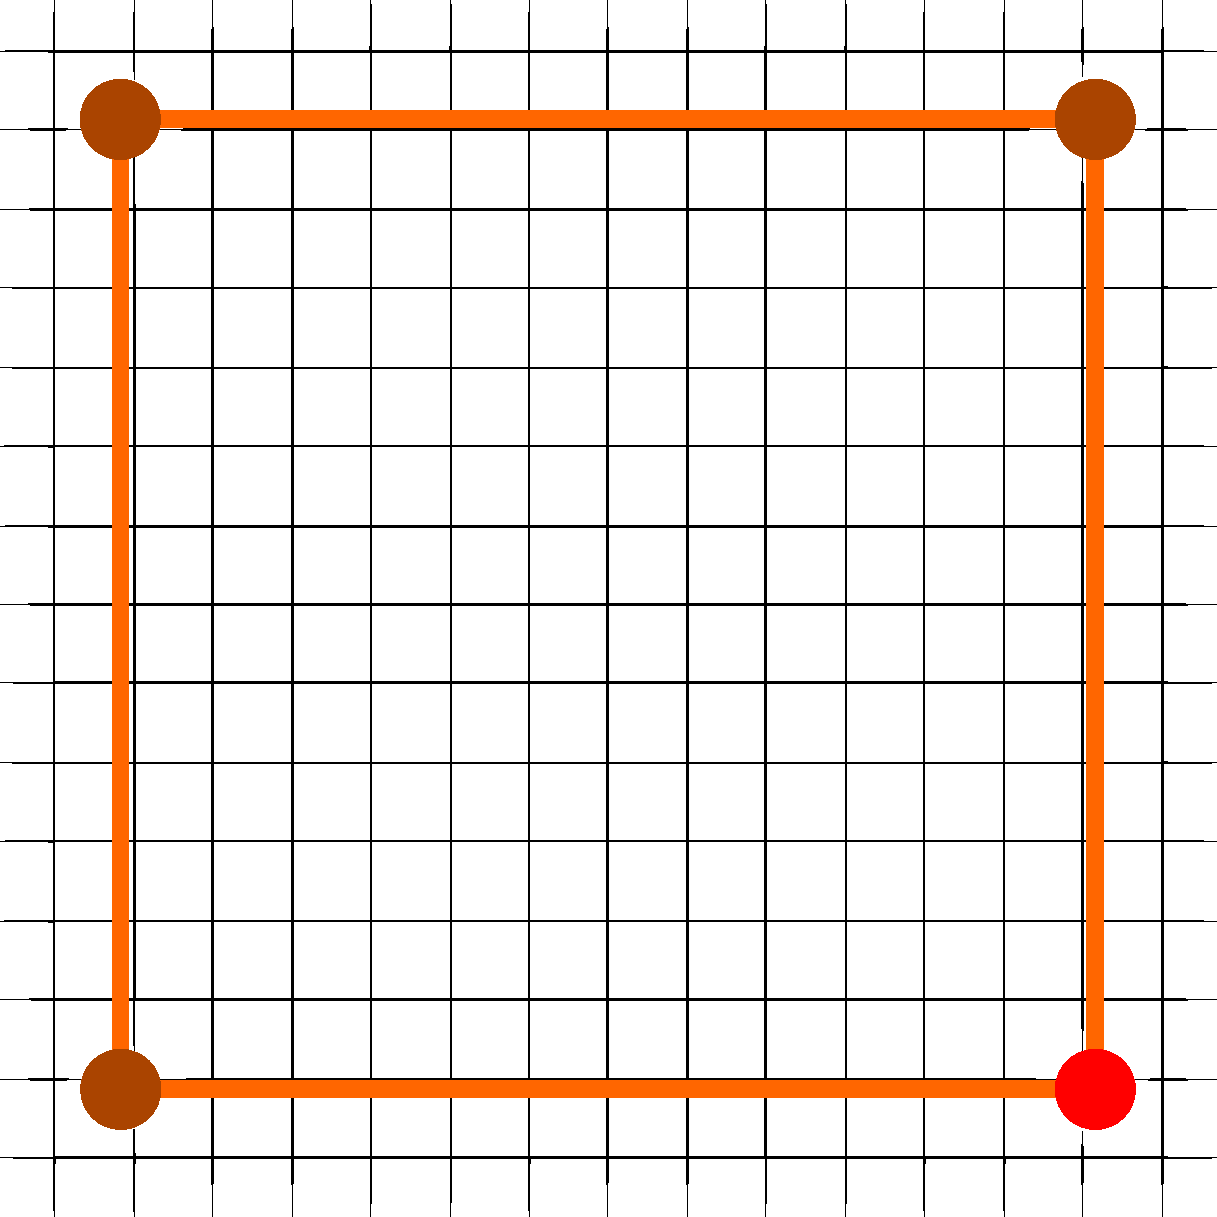
\includegraphics[scale=1.5]{Deformation-Interieur-1Sommet-Avant}
      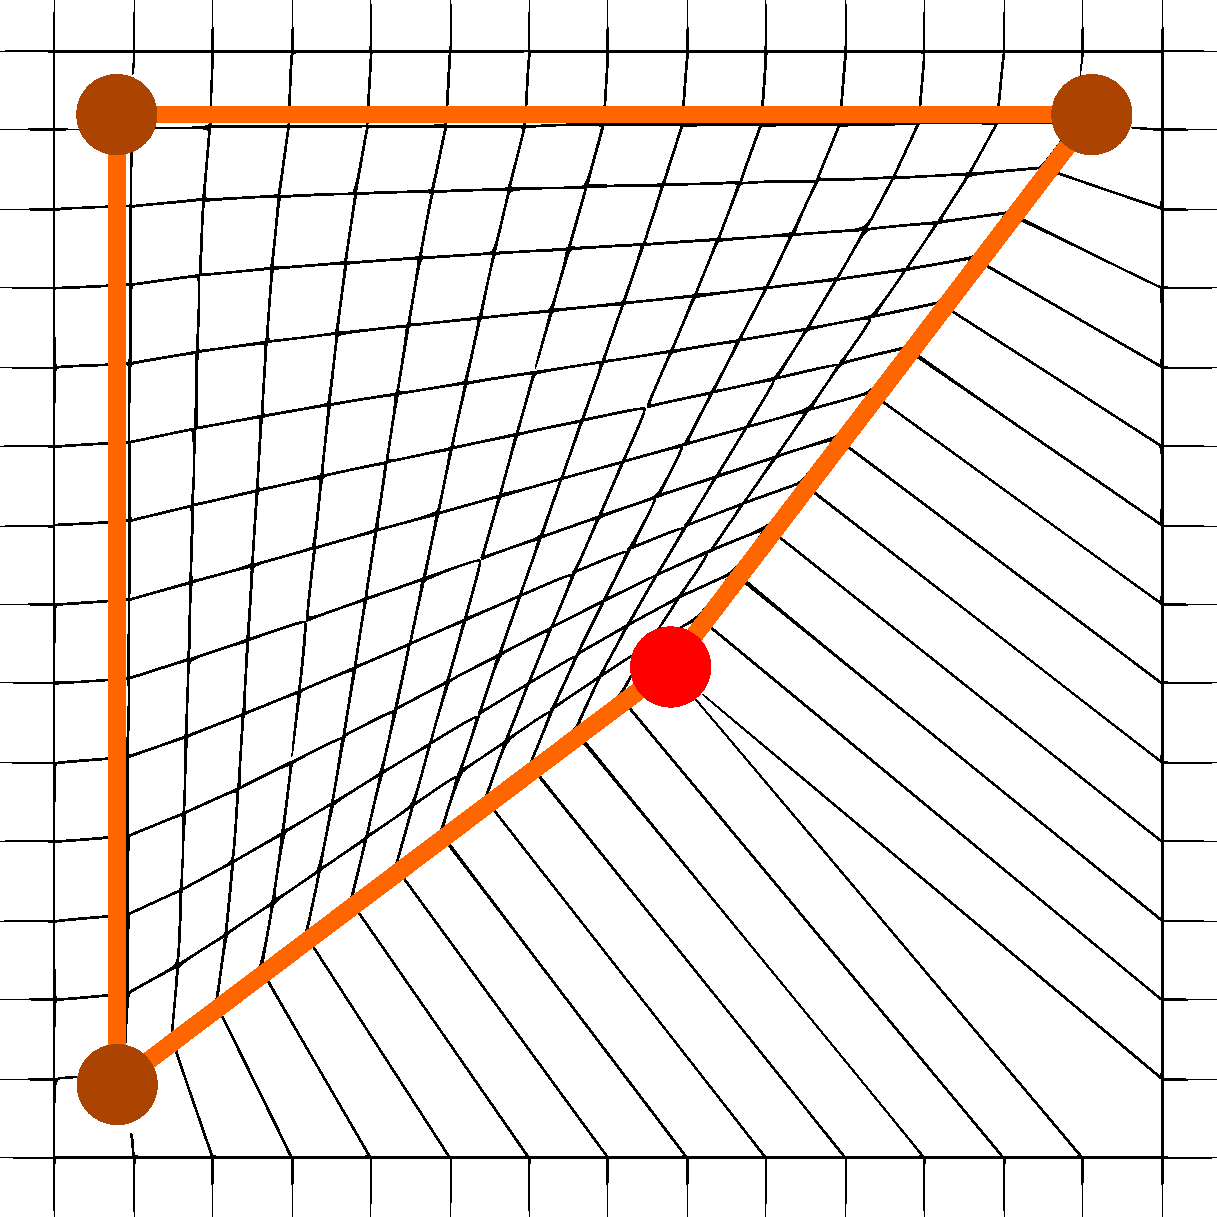
\includegraphics[scale=1.5]{Deformation-Interieur-1Sommet-Apres}
    }

    \caption[Problème de continuité déformation naïve] {Visualisation des
problèmes de continuité lorsque seuls les points à l'intérieur de la cage sont
déformés. Le bord de la cage est représenté en orange, le modèle est
représenté par une grille régulière en noir. Le sommet en rouge représente le
sommet déplacé. A gauche le modèle avant déformation, à droite le même modèle
après déformation.}

    \label{MELVI}
  \end{center}
\end{figure}

En considérant des coordonnées pour les points de l'espace à la fois à
l'intérieur et à l'extérieur de la cage le problème vient de la dérivabilité
de la fonction résultant de la déformation. Plus précisément, pour les MVC et
GC la fonction de déformation est définie dans $\mathbb{R}^2$ et est
$C^{\infty}$ partout sauf au niveau des sommets de la cage où elle n'est que
$C^0$ (d'après \cite{LS08}). La déformation engendrée n'est pas visuellement lisse autour des
sommets de la cage. Quant aux HC, elles ne sont définies qu'à l'intérieur de
la cage où elles sont $C^{\infty}$, il n'y a donc aucun moyen de déformer
l'extérieur de la cage de cette manière.

Notre objectif est d'obtenir une fonction de déformation, définie par une
cage, qui soit au moins $C^1$ partout (visuellement lisse) et dont la zone
d'influence soit limitée.

Plutôt que de mettre en place une nouvelle méthode de calcul de coordonnées
ayant les propriétés que nous souhaitons, ce qui au demeurant serait un sujet
de recherche en soi, nous nous intéressons plutôt à la réutilisation des
méthodes de calcul existantes.

\subsubsection{Principe}

Nous considérons deux cages là où les travaux antérieurs n'en considéraient
qu'une seule. Nous appelons \textit{cage de contrôle} la cage avec laquelle
l'utilisateur interagit pour réaliser les déformations. Nous appelons
\textit{cage d'influence} la cage qui définit la zone d'influence (points de
l'espace qui sont sous l'influence de la déformation). La cage d'influence est
homothétique à la cage de contrôle et contient strictement cette dernière
(Figure \ref{MELDou}).

\begin{figure}[ht]
  \begin{center}
    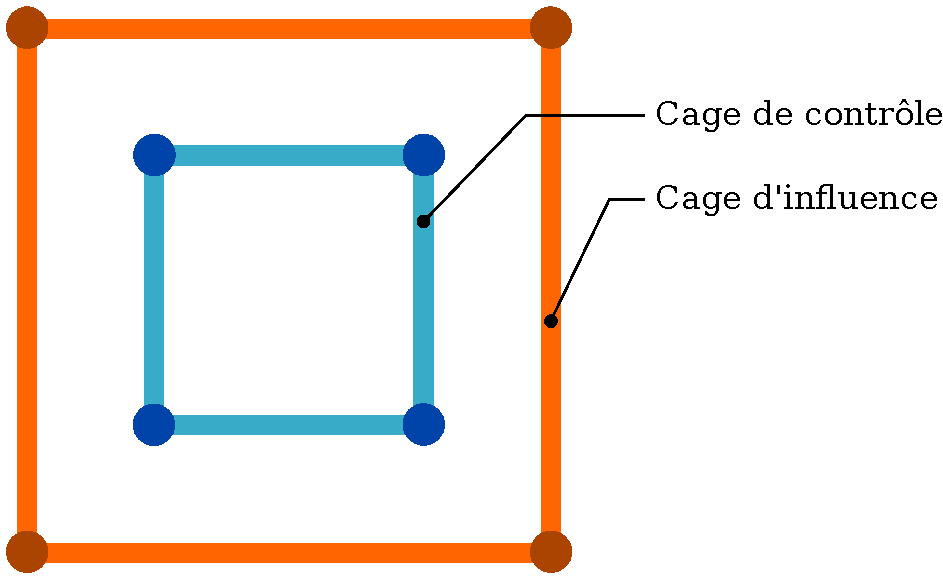
\includegraphics[scale=0.5]{chapter3-doubleCage-description-pstricks}

    \caption[Disposition des cages de contrôle et d'influence] {Disposition
des deux cages. En bleu la cage de contrôle, en orange la cage d'influence.}

    \label{MELDou}
  \end{center}
\end{figure}

Avec cette disposition, l'extérieur de la cage de contrôle peut-être
interprêté comme l'intérieur de la cage d'influence. Il se trouve que les
coordonnées MVC sont $C^{\infty}$ à l'intérieur de la cage d'influence (par
définition), les déformations qui ont lieu à l'intérieur de celle-ci sont donc
visuellement lisses. On introduit une notion de hiérarchie de déformation, où
la modification de la position des sommets de la cage de contrôle va modifier
la position des sommets de la cage d'influence, qui elle- même va modifier
l'espace contenu en son intérieur, grâce aux méthodes de calcul de coordonnées
existantes (MVC, HC, GC). \\

\subsubsection{Hiérarchie de la déformation}

Il faut maintenant établir un lien entre les deux cages, afin que la
modification de la position des sommets de la cage de contrôle affecte la
position des sommets de la cage d'influence.

Une première idée est d'utiliser des coordonnées barycentriques généralisées
pour évaluer la position de chacun des sommets de la cage d'influence comme
une combinaison linéaire pondérée des positions des sommets de la cage de
contrôle. Cette technique pose un problème quant à la localité de la
déformation : la modification de la position d'un sommet de la cage de
contrôle modifie la position de tous les sommets de la cage d'influence
(Figure \ref{MELDMV}). Nous voulons que les points les plus éloignés du sommet
modifié soient le moins affectés par la déformation engendrée. La modification
de la position d'un sommet de la cage de contrôle doit donc modifier le moins
de sommets de la cage d'influence.

\begin{figure}[ht]
\begin{center}
  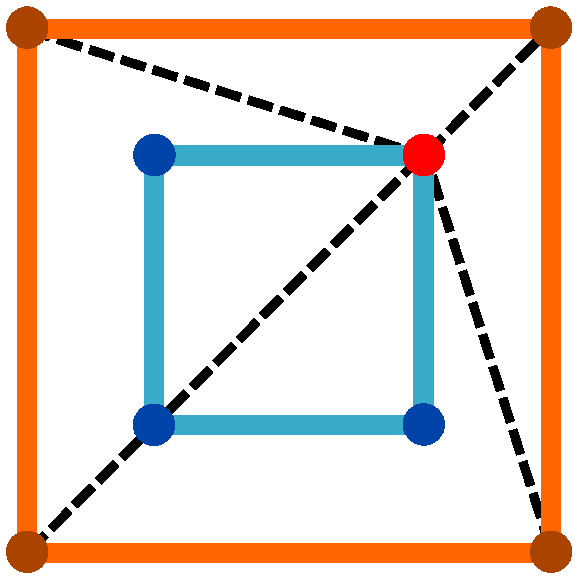
\includegraphics[scale=0.5]{chapter3-doubleCage-MVC-avant-pstricks}
  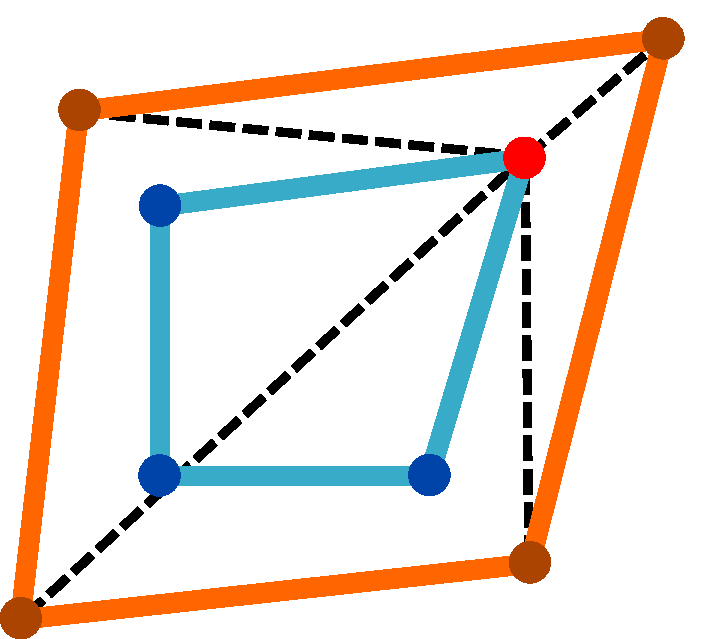
\includegraphics[scale=0.5]{chapter3-doubleCage-MVC-apres-pstricks}

  \caption[Lien double-cage MVC] {Lien entre les cages de contrôle et
d'influence utilisant les coordonnées MVC. Les pointillés noirs représentent
le lien entre un sommet de la cage de contrôle et les sommets de la cage
d'influence.On peut remarquer que la position de tous les sommets de la cage
d'influence est modifiée à la modification de la position du sommet en rouge.}

  \label{MELDMV}
\end{center}
\end{figure}

A la place, on peut proposer que chaque sommet de la cage d'influence soit lié à
un seul sommet de la cage de contrôle. Etant donné que l'on construit la cage
d'influence comme une version mise à l'échelle de la cage de contrôle, on peut
facilement lier les sommets de la cage de contrôle à leur homologues "mis à
l'échelle" de la cage d'influence. Ainsi, quand on modifie la position d'un
sommet de la cage de contrôle, un seul sommet de la cage d'influence est
déplacé (Figure \ref{MELHie}).

On définit donc le lien comme un vecteur $\overrightarrow{v}$ représentant la
différence de position entre un sommet de la cage d'influence $v_{inf}$ par
rapport au sommet de la cage de contrôle $v_{ctrl}$ auquel il est associé :

\begin{displaymath}
  \overrightarrow{v} = v_{inf}-v_{ctrl}
\end{displaymath}

\begin{figure}[ht]
\begin{center}
  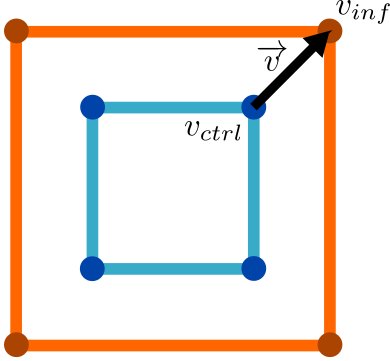
\includegraphics[scale=0.5]{chapter3-doubleCage-hierarchie-avant-pstricks}
  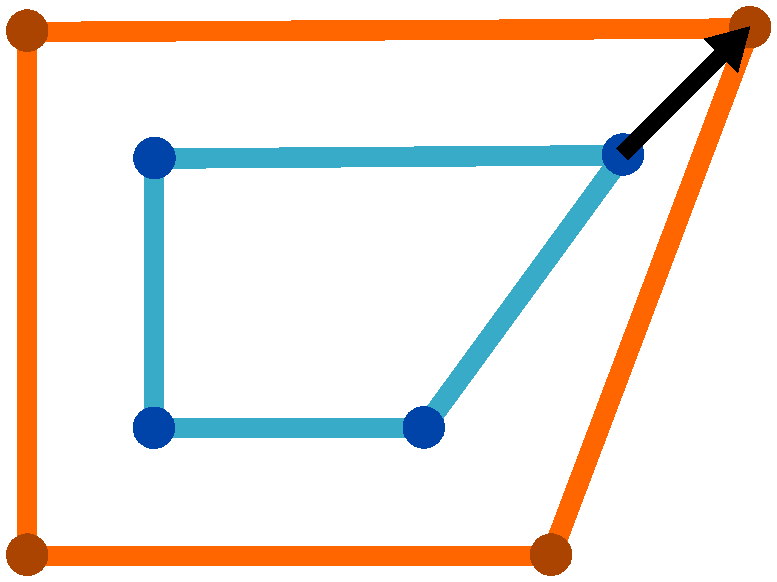
\includegraphics[scale=0.5]{chapter3-doubleCage-hierarchie-apres-pstricks}

  \caption[Association des cages de contrôle et d'influence] {Modification de
la position du sommet de la cage d'influence $v_{inf}$ associé au sommet de la
cage de contrôle déplacé $v_{ctrl}$. A gauche les cages avant déformation, à
droite les cages après déformation. En bleu la cage de contrôle, en orange la
cage d'influence et en noir le vecteur $v$.}

  \label{MELHie}
\end{center}
\end{figure}

\subsubsection{Atténuation de la déformation}

Pour l'instant, la déformation souffre toujours de problème de continuité au
niveau du bord de la cage d'influence. Pour corriger ce problème, nous allons
progressivement atténuer la déformation appliquée, en fonction de la distance
d'un point de l'espace au bord de la cage d'influence.

Pour atténuer la déformation nous avons choisi d'interpoler linéairement la
position qu'un point de l'espace avait initialement (au temps d'association)
avec la position qu'il devrait avoir avec une déformation classique:

\begin{equation}
  T_{d}(p) = \gamma(p) p + (1-\gamma(p)) T(p)
\end{equation}

où $p$ correspond à la position initiale du point, $T(p)$ la position que ce
point aurait après la déformation et $T_{d}(p)$ la position finale du point.

\textbf{Distance au bord de la cage d'influence :}

Nous avons choisi d'interpréter la fonction $\gamma$ comme représentant la
distance du point $p$ au bord de la cage d'influence. Nous utilisons les
coordonnées que nous avons déjà calculé pour chacun des points de l'espace par
rapport aux sommets de la cage d'influence. Ce choix a l'avantage de ne pas
nécessiter de réaliser des calculs supplémentaires. On établit que la distance
au bord $d_{inf}(p)$ doit être égale au produit des poids associés à chacune
des arêtes de la cage d'influence. Où le poids associé à une arête $e_i$
correspond à la somme des poids associés aux sommets incidents $v_j$ à cette
arête :

\begin{equation}
  d_{inf}(p) = \prod_{e_i \in c_{inf}} (1 - \sum_{v_j \in e_i} \lambda_j(p))
  \label{MELInf}
\end{equation}

Ce calcul s'inspire de la notion de "boundary weight function" de
\cite{GPCP13}, où les auteurs utilisaient cette fonction pour évaluer la
distance d'un point à chacune des arêtes d'une cage.

$0 \leq d_{inf}(p) \leq \frac{2}{n}^n$, donc pour 

Cette fonction n'est pas dérivable au bord de la cage d'influence (Figure
\ref{MELAtN}).

\begin{figure}[ht]
\begin{center}
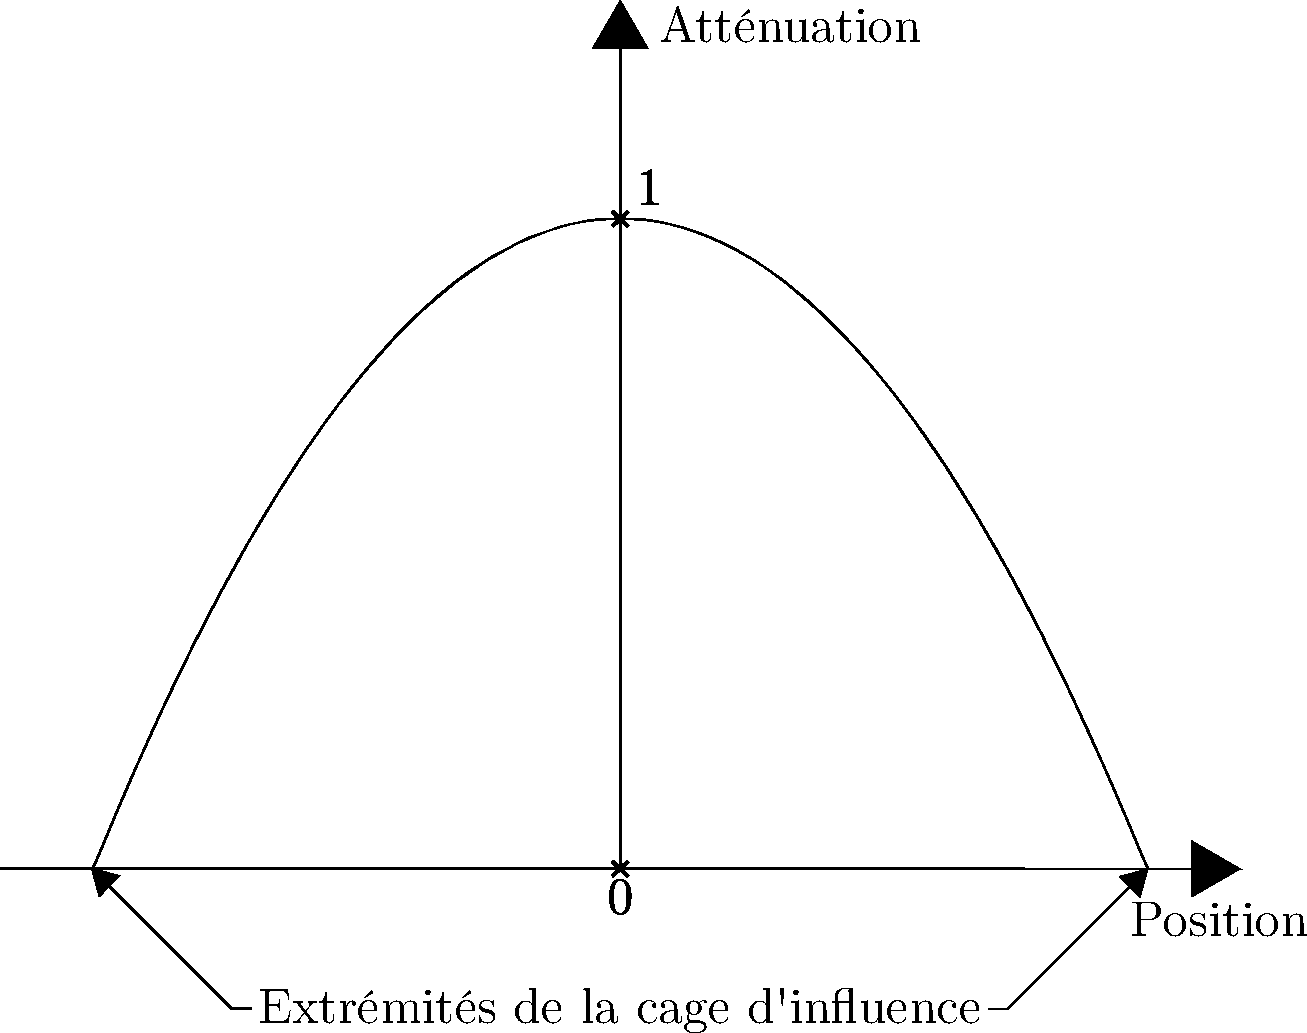
\includegraphics[scale=0.5]{Fonction-Attenuation-Sans}

\caption[Fonction d'atténuation (non lissée)] {Vue en coupe de la fonction
d'atténuation $d_{inf}(p)$ (non lissée). On peut remarquer que la fonction
n'est pas dérivable au niveau du bord de la cage d'influence.}

\label{MELAtN}

\end{center}
\end{figure}

Nous utilisons donc une fonction $f_h(x)$, paramétrisée par $h \in ]0, 1]$,
permettant de lisser les valeurs des distances des points de l'espace au bord de
la cage d'influence. Cette fonction doit satisfaire $f_h(0) = f_h'(0) =
f_h'(1) = 0$, $f_h(x)=1$ pour $x \geq h$ et $f'_h(x) \geq 0$. L'idée vient du
travail de \cite{GPCP13}, où ils utilisaient cette fonction pour lisser les
valeurs de distance d'un point à une arête de la cage. Les auteurs proposaient
plusieurs fonctions avec des comportements similaires, nous en avons donc
gardé une arbitrairement :

\begin{equation}
  f_h(x) = \frac{1}{2} sin(\pi(\frac{x}{h} - \frac{1}{2})) + \frac{1}{2}
\end{equation}

\textbf{Calcul du paramètre $h$ :}

Il faut évaluer la valeur de $h$ de manière à ce que ce paramètre représente
la différence de taille entre la cage de contrôle et la cage d'influence. On
souhaite que la déformation ne soit pas atténuée pour l'ensemble des points de
l'espace à l'intérieur de la cage de contrôle. On va donc définir $h$ comme
étant la distance minimale à partir de laquelle la déformation ne doit pas
être atténuée. Cette valeur correspond à la plus courte distance d'un point de
l'espace (inclus dans la cage de contrôle) au bord de la cage d'influence.
Plus précisément, il s'agit exactement de la valeur de distance du sommet de
la cage de contrôle le plus proche du bord de la cage d'influence. Il nous
suffit donc d'évaluer la valeur de distance en chacun des sommets de la cage
de contrôle par rapport au bord de la cage d'influence et de les comparer afin
de trouver la distance minimale :

\begin{equation}
  h = \min_{\forall v_{ctrl}} d_{inf}(v_{ctrl}).
\end{equation}

On peut maintenant écrire $\gamma(p)$ comme étant le résultat du lissage de la
fonction \ref{MELInf} :

\begin{equation}
  \gamma(p) = f_h(d_{inf}(p)).
\end{equation}

En regardant la fonction $\gamma(p)$, on peut remarquer qu'il n'y a plus de
problèmes de continuité au niveau du bord de la cage d'influence (Figure
\ref{MELAtL}).

\begin{figure}[ht]
\begin{center}
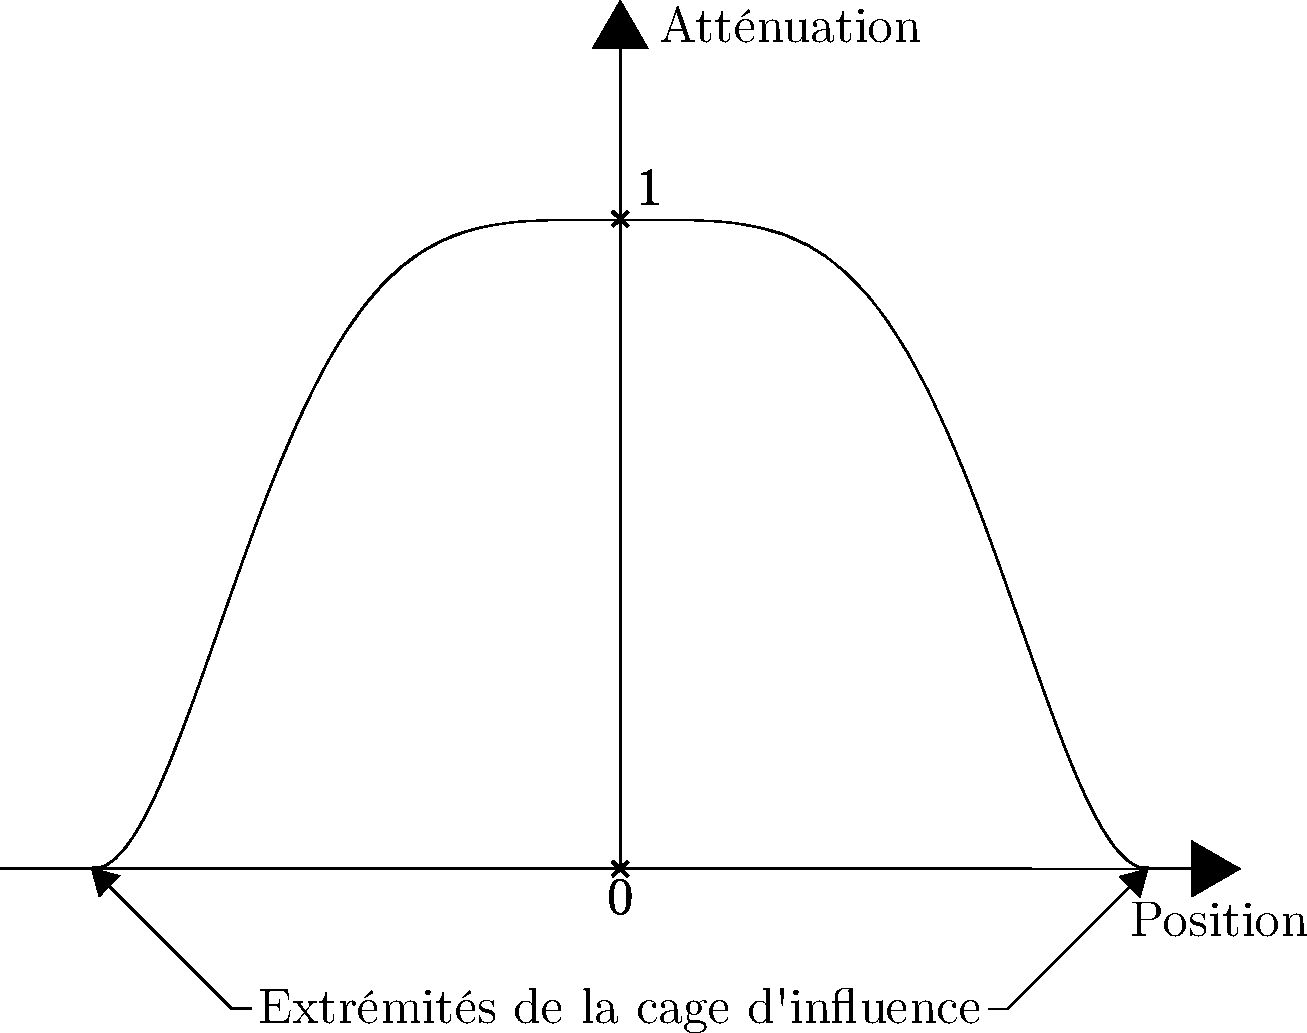
\includegraphics[scale=0.5]{Fonction-Attenuation-Avec}

\caption[Fonction d'atténuation $\gamma$(p)] {Vue en coupe de la fonction
d'atténuation $\gamma$(p). On peut remarquer que la fonction est maintenant
dérivable au niveau du bord de la cage d'influence.}

\label{MELAtL}

\end{center}
\end{figure}

Plus la différence de taille entre la cage de contrôle et la cage d'influence
est grande, plus l'atténuation de la déformation est douce (Figure
\ref{MELBou}).

\begin{figure}[ht]
  \begin{center}
    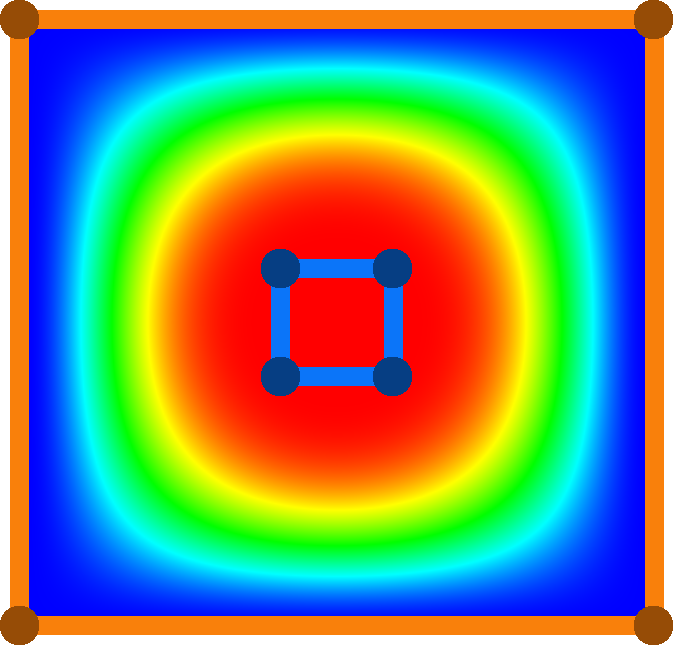
\includegraphics[scale=0.2]{BoundaryWeightFunction-Petite}
    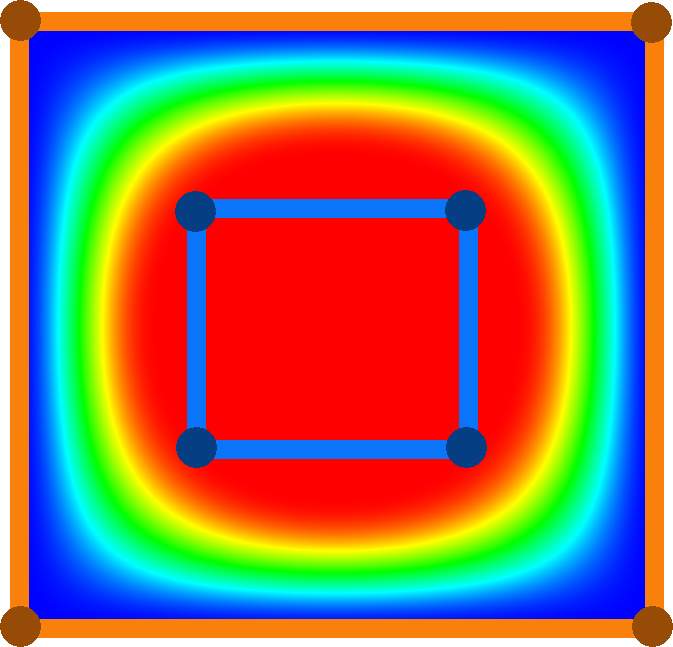
\includegraphics[scale=0.2]{BoundaryWeightFunction}
    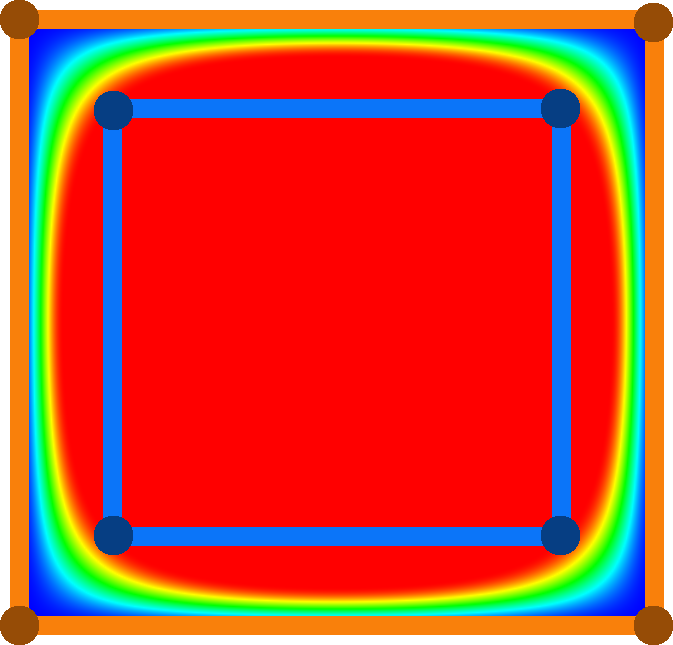
\includegraphics[scale=0.2]{BoundaryWeightFunction-Grande}

    \caption[Variation de l'atténuation de la déformation] {Variation de
l'atténuation de la déformation. La couleur varie du rouge (atténuation nulle)
au bleu (atténuation totale). De gauche à droite on peut voir la variation
pour différentes tailles de cage de contrôle.}

    \label{MELBou}
  \end{center}
\end{figure}

Ci-dessous l'algorithme représentant l'étape de déformation du modèle avec
atténuation de l'influence de la déformation: \\

\fbox{\begin{minipage}{0.9\textwidth}
  \begin{algorithm}[H]
  \KwIn{$pos$, $pos_{init}$ : tableau de tableau de réels}
  \ForEach{point de l'espace p}
  {
    $pos$[p] $\leftarrow$ [0,0]\; 
      \ForEach{sommet v de la cage d'influence c}
      {
        $pos$[p] $\leftarrow$ $pos$[p] + $\lambda_v(p)$ * $pos$[v] 
        * $d_{inf}(c, p)$\;
        $pos$[p] $\leftarrow$ $pos$[p] + $\lambda_v(p)$ * $pos_{init}$[v] 
        * (1-$d_{inf}(c, p)$)\;
      }
  }
  \caption{Déformation avec zone d'influence modifiée}
  \end{algorithm}
\end{minipage}} \\

Pour simplifier les écritures dans la suite du travail, nous nous référons à
ce nouvel outil (composé d'une cage de contrôle et d'une cage d'influence)
comme étant l'outil \textit{cage de contrôle d'influence} ou \textit{cage
coninf}.

\begin{figure}[ht]
  \begin{center}
    
\includegraphics[scale=0.3]{Deformation-Capricorne-Avant}
    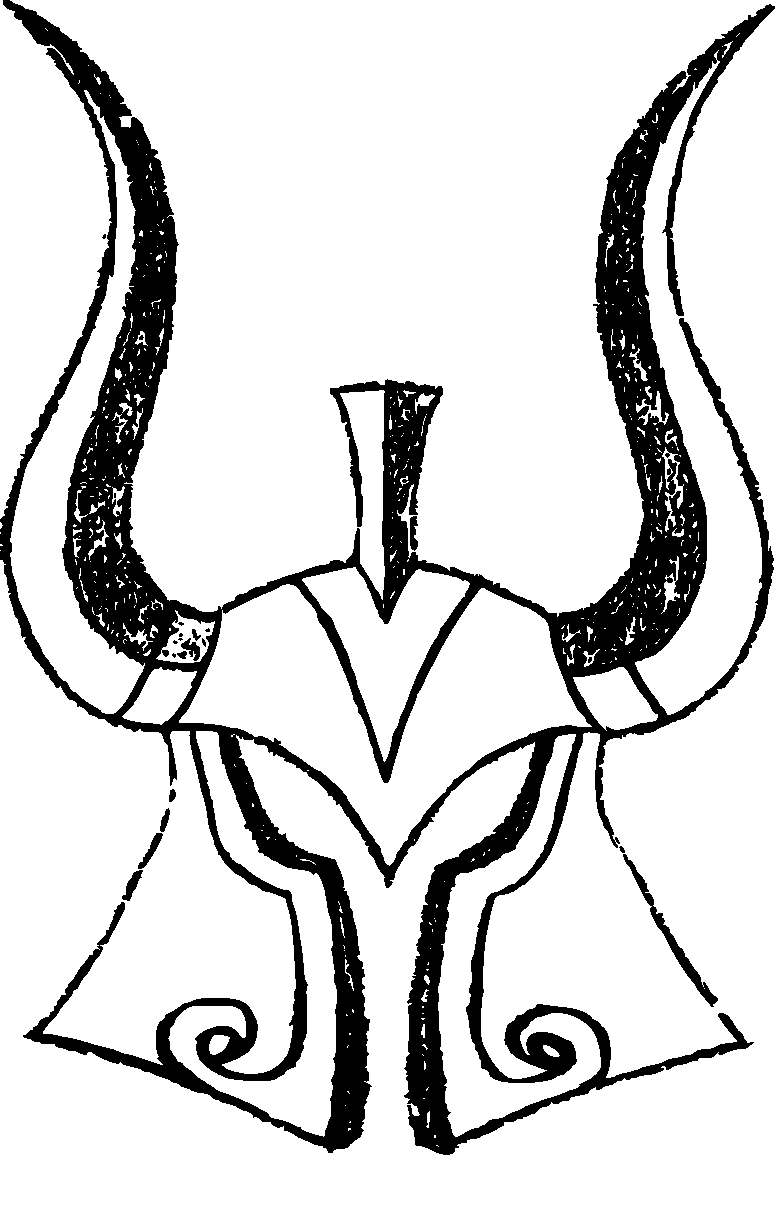
\includegraphics[scale=0.3]{Deformation-Capricorne-Apres}

    \caption[Exemple de déformation cage de contrôle d'influence] {Exemple de
déformation avec une cage de contrôle d'influence. A gauche le casque et la
cage coninf au temps d'association, à droite après modification de la position
des sommets de la cage de contrôle. On peut remarquer que la partie haute du
casque (cimier) n'a pas été modifiée par la déformation.}

  \end{center}
\end{figure}

\subsection{Combinaison des déformations}

Maintenant que nous avons établi un outil de déformation local, nous voulons
combiner plusieurs cages coninf sur un même modèle (Figure \ref{MELMC}).
L'objectif de cette partie consiste à trouver une formule de mélange
permettant la modification de la position d'un point de l'espace par rapport à
plusieurs cages coninf. De manière à ce que la déformation résultant du
mélange soit visuellement lisse.

\begin{figure}[ht]
  \begin{center}
    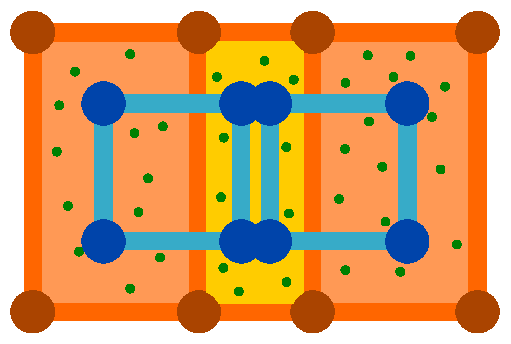
\includegraphics[scale=1]{chapter3-doubleCage-melange-pstricks}

    \caption[Mélange de cages de contrôle d'influence] {Exemple de
configuration de deux cages de contrôle d'influence se chevauchant. Les points
de l'espace (en vert) appartenant à la zone en jaune sont sous l'influence des
deux cages à la fois}

    \label{MELMC}
  \end{center}
\end{figure}

Combiner les déformations revient à établir une combinaison linéaire pondérée
de l'influence de chaque cage coninf. Pour établir la valeur du coefficient
associé à chaque cage, il faut trouver un critère permettant de classer les
cages selon l'importance de la déformation à appliquer. Le critère que nous
décidons d'envisager est celui de distance. En effet, intuitivement, plus
un point de l'espace est proche du centre d'une cage coninf, plus on aimerait
que cette cage influe sur la déformation de ce point. Autrement dit, on va
regarder la proximité d'un point de l'espace au centre de chaque cage coninf à
laquelle il appartient.

Comparer la proximité au centre d'une cage coninf revient au même que de
comparer l'éloignement au bord de la cage d'influence. Ainsi, on peut
réutiliser les valeurs de distance au bord de la cage d'influence $d_{inf}(p)$
pour connaître la proximité d'un point au centre d'une cage coninf. Ces
distances étant relatives à chaque cage, il est nécessaire de les normaliser
afin de pouvoir les comparer entre elles :

\begin{displaymath}
  D_{inf_i}(p) = \frac{d_{inf_i}(p)}{\sum_{j=0}^n d_{inf_j}(p)}, 
\end{displaymath}

où $D_{inf_i}(p)$ correspond à la distance normalisée du $p$ par rapport au
bord de la cage d'influence constituant la cage coninf $i$.

On peut maintenant définir une fonction de mélange se basant sur la proximité
d'un point de l'espace au centre des différentes cages coninf auquel il
appartient :

\begin{displaymath}
  T_{mel}(p) = \sum_{i=0}^n D_{inf_i}(p) T_{d_i}(p).
\end{displaymath}

Ci-dessous l'algorithme représentant l'étape de déformation du modèle avec le
mélange des déformations: \\

\fbox{\begin{minipage}{0.9\textwidth}
\begin{algorithm}[H]
\KwData{$sumD_{inf}$, $D_{inf}$: réel}
\KwIn{$pos$, $pos_{init}$ : tableau de tableau de réels}
\ForEach{point de l'espace p}
{
  $sumD_{inf}$ $\leftarrow$ 0\;
  \ForEach{cage d'influence c associée à p}
  {
    $sumD_{inf}$ $\leftarrow$ $sumD_{inf}$ + $d_{inf}(c, p)$\;
  }
  $pos$[p] = [0,0]\; 
  \ForEach{cage d'influence c associée à p}
  {
    $D_{inf}$ $\leftarrow$ $d_{inf}(c, p)$ / $sumD_{inf}$\;
    \ForEach{sommet v de c}
    {
      $pos$[p] $\leftarrow$ $pos$[p] + $\lambda_v(p)$ * $pos$[v] 
      * $d_{inf}(c, p)$ * $D_{inf}$\;
      $pos$[p] $\leftarrow$ $pos$[p] + $\lambda_v(p)$ * $pos_{init}$[v] 
      * (1-$d_{inf}(c, p)$) * $D_{inf}$\;
    }
  }
}
\caption{Mélange des déformations}
\end{algorithm}
\end{minipage}} \\

\begin{figure}[ht]
  \begin{center}
    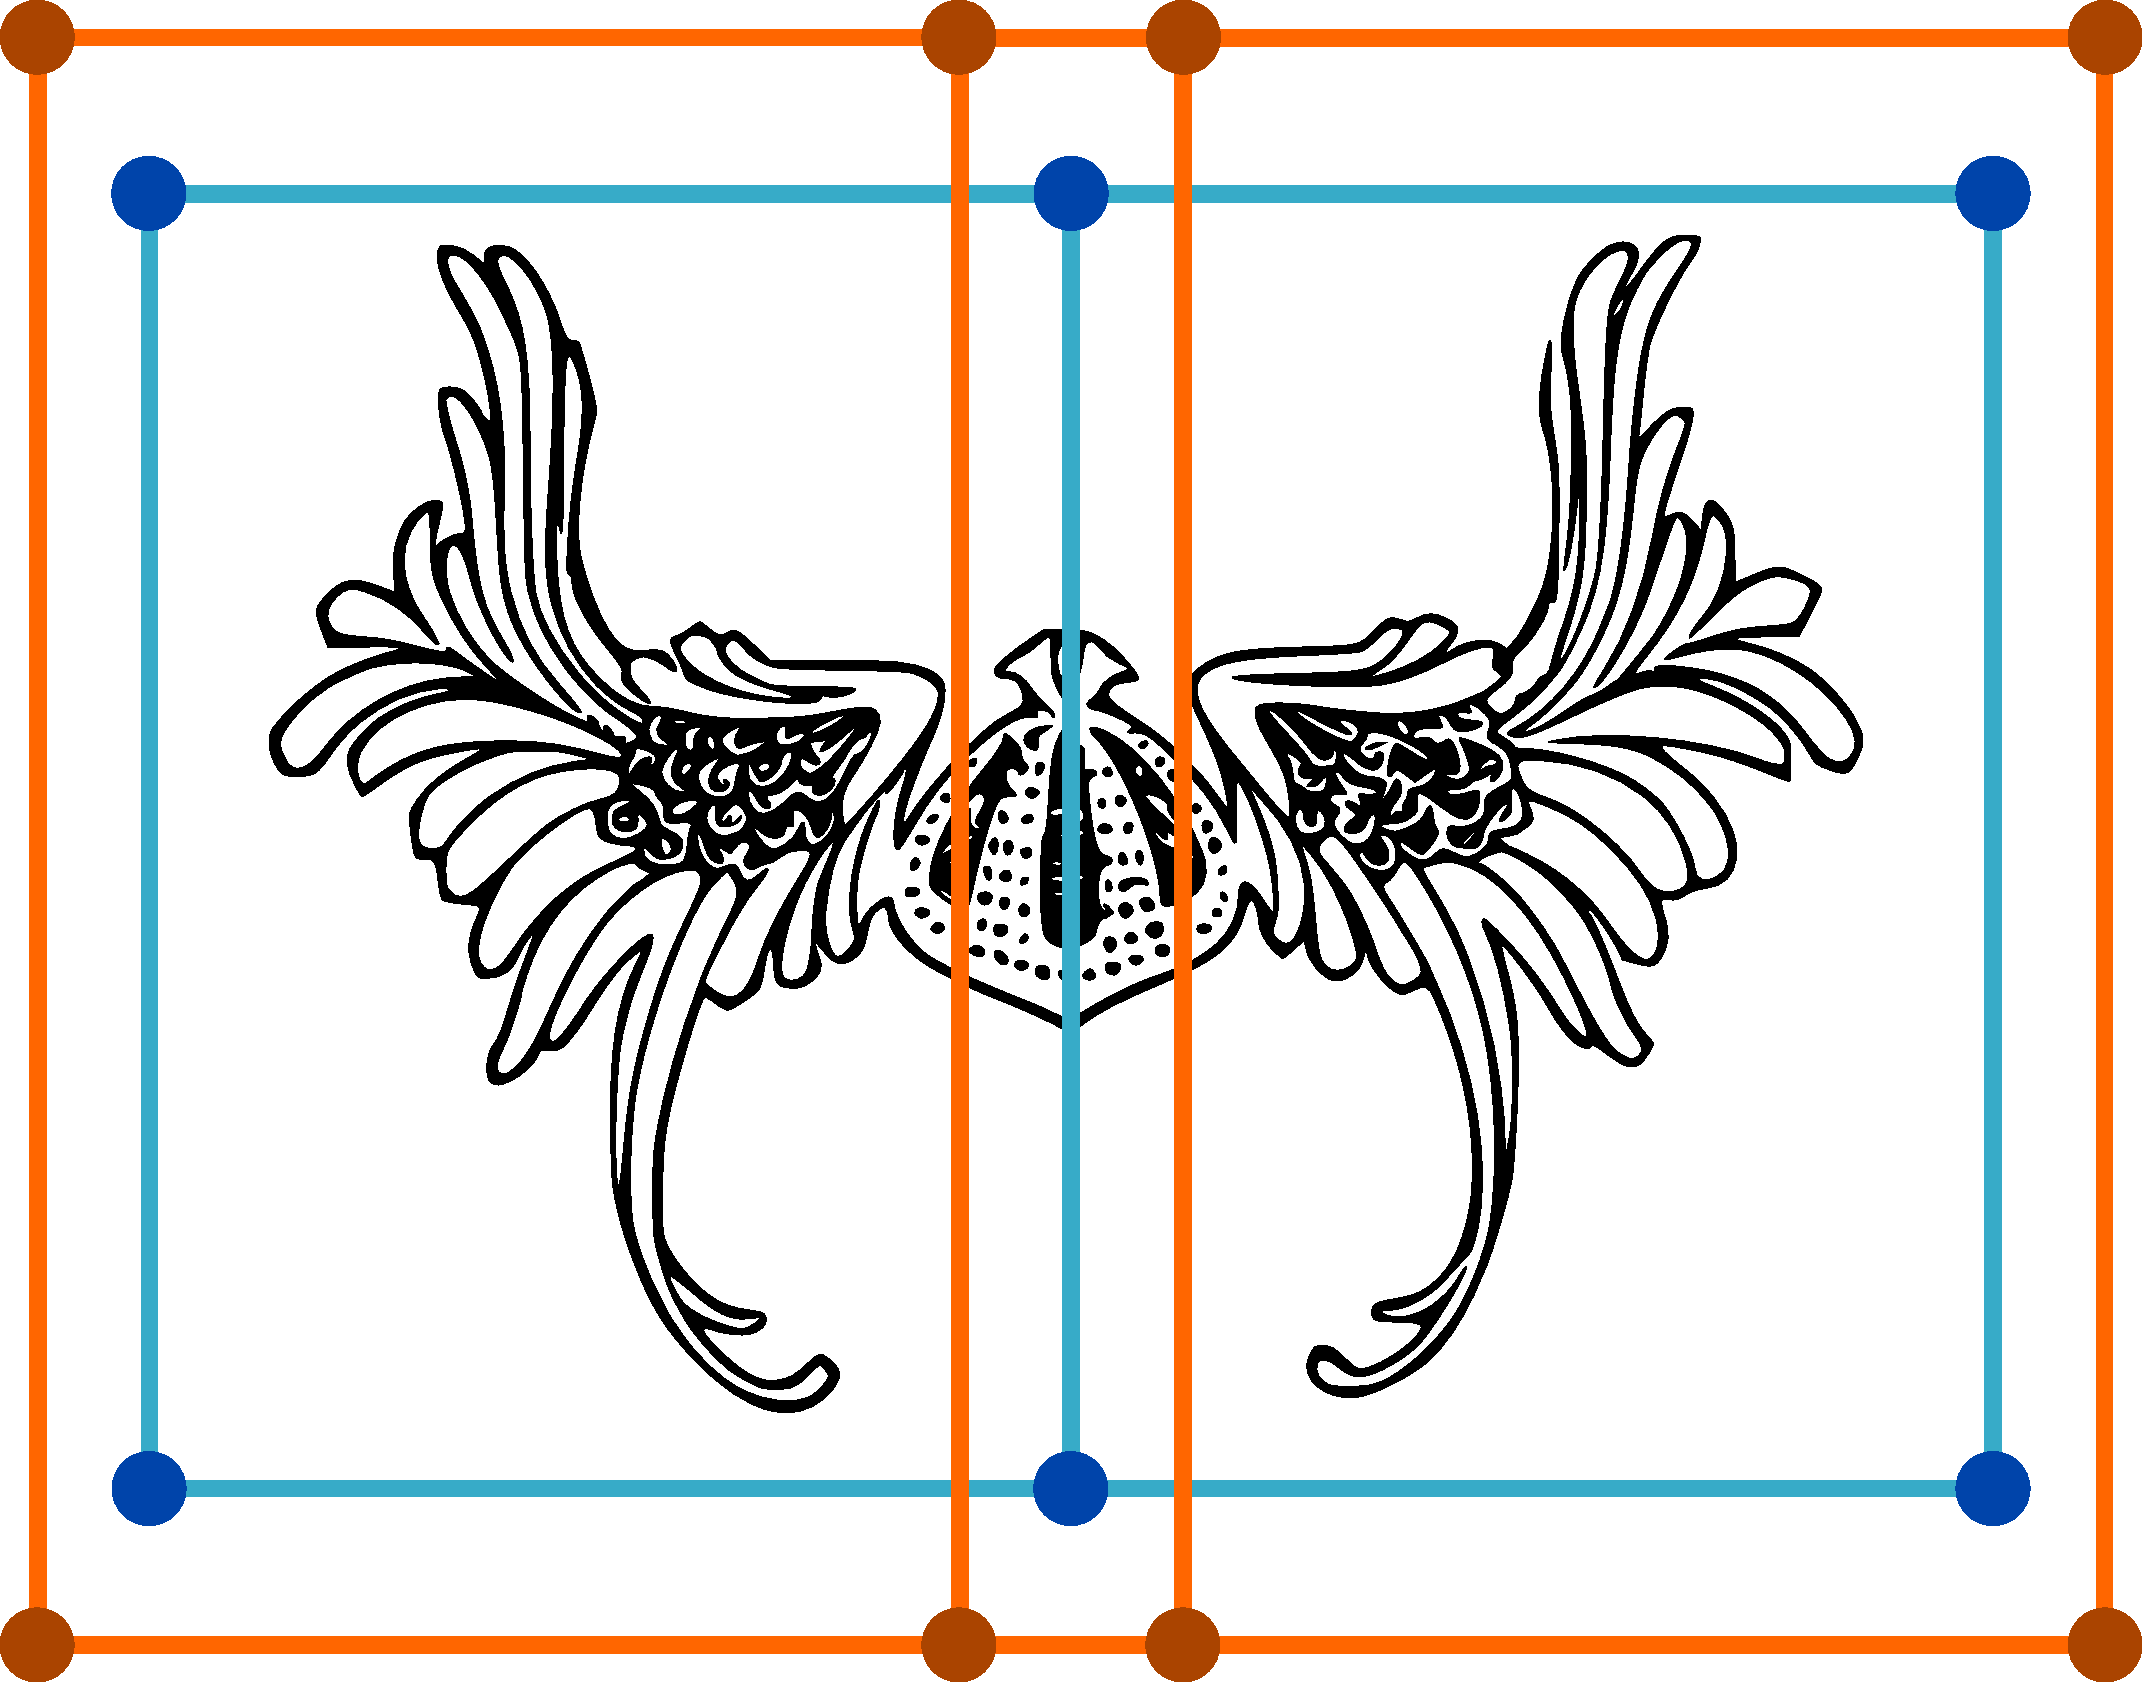
\includegraphics[scale=0.3]{Deformation-Viking-Avant}
    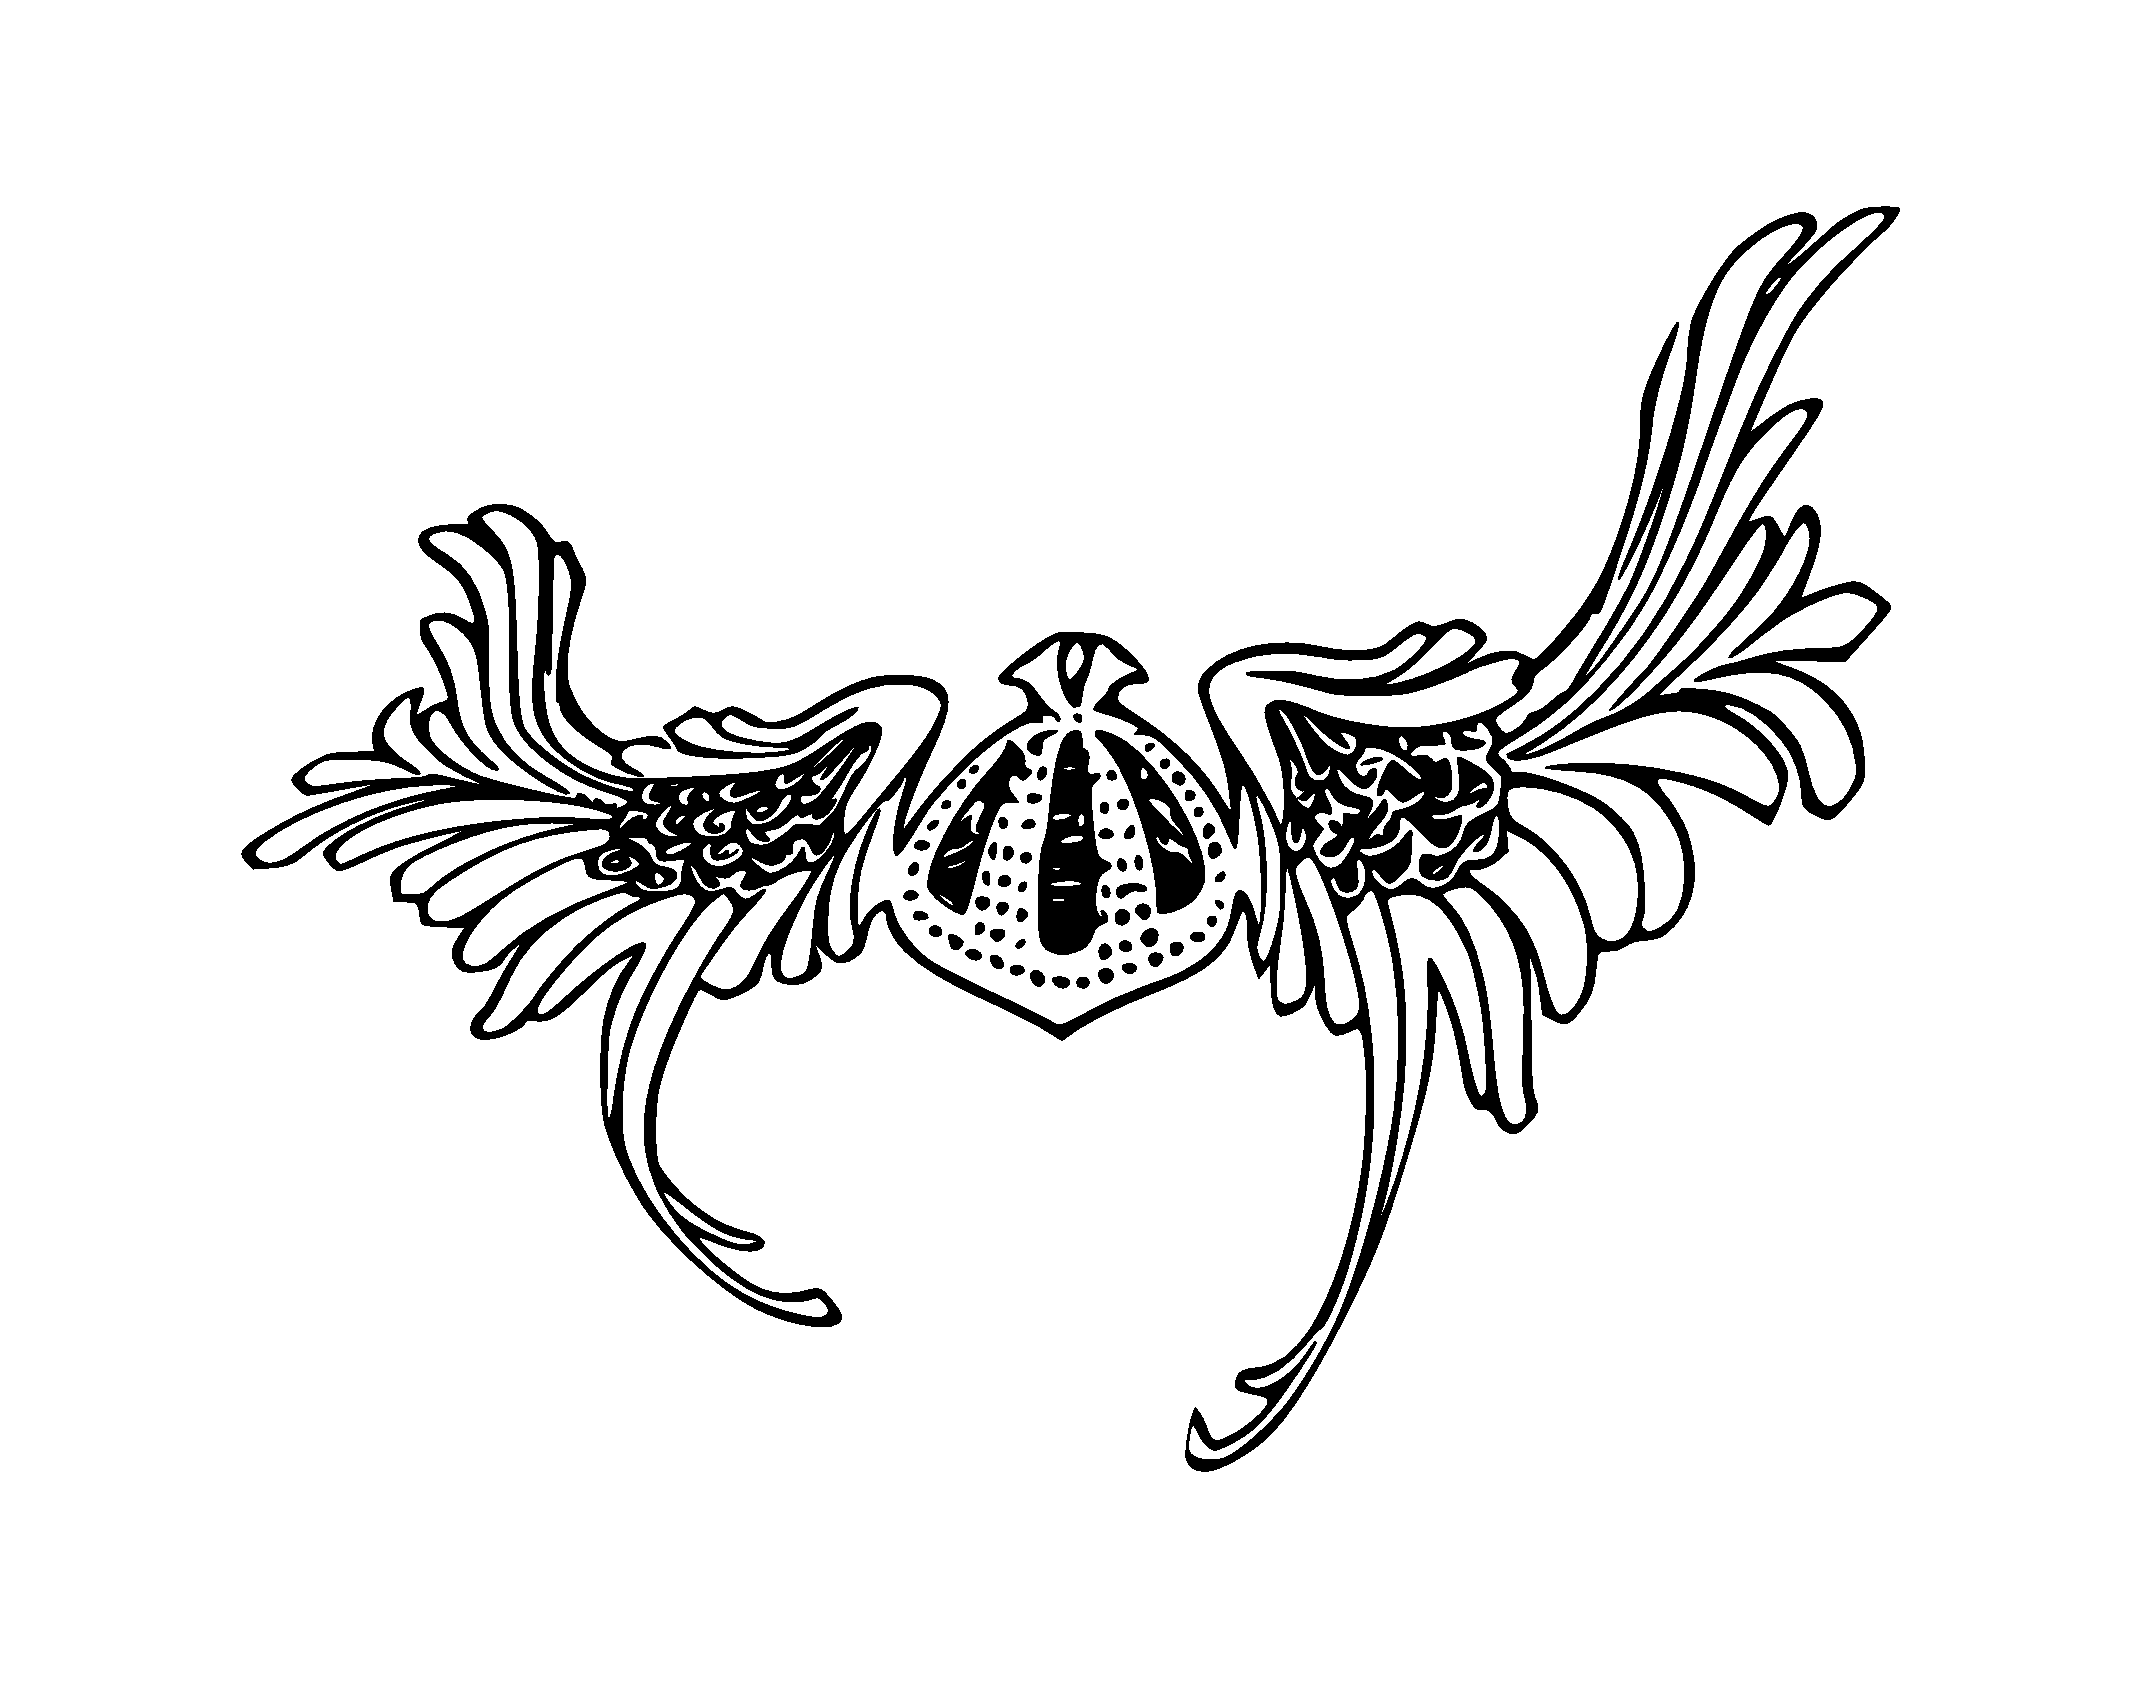
\includegraphics[scale=0.3]{Deformation-Viking-Apres}

    \caption[Exemple de déformation cage de contrôle d'influence] {Exemple de
déformation avec deux cages de contrôle d'influence (en bleu les cages de
contrôle, en orange les cages d'influence) où les cages de contrôle ont été
collées ensembles le long d'une arête commune. A gauche le casque avant
déformation, à droite après modification de la position des sommets des deux
cages de contrôle.}

  \end{center}
\end{figure}


%!TEX root = ../thesis.tex

% \pagebreak[4]
% \hspace*{1cm}
% \pagebreak[4]
% \hspace*{1cm}
% \pagebreak[4]

\chapter{Extensions}

\graphicspath{ {Chapter4/Chapter4Figs/PNG/}
  {Chapter4/Chapter4Figs/PDF/} {Chapter4/Chapter4Figs/} }

Dans le dernier chapitre, nous avons vu une nouvelle méthode permettant
combiner des outils de déformation à base de cage. Cette méthode utilise un
nouveau type d'outil, la cage de contrôle d'influence. Cet outil est composé
de deux cages. L'une dite d'influence, elle délimite la zone de l'espace
sous l'influence de la déformation. L'autre dite de contrôle, elle permet à
l'utilisateur de contrôler la déformation à appliquer.

Ce sujet se tourne vers la création d'un outil multidimensionnel de
déformation. Mais nous n'avons pour l'instant travaillé que sur des
déformation à base d'outils de dimension 2. Il est naturel de se demander
comment notre méthode pourrait être étendue à des outils de dimensions
différentes. Deux approches sont possibles pour généraliser ce travail :

\begin{enumerate}
\item Modifier la nature de la cage de contrôle
\item Mélanger des outils existants avec cette méthode
\end{enumerate}

\section{Modification de la nature de la cage de contrôle}

Nous avions choisi de travailler avec une cage comme outil de contrôle puisque
nous voulions une méthode de mélange d'outils de déformation à base de cage.
Mais rien ne nous empêche de changer la nature de cette cage de contrôle. Pour
généraliser un peu plus ces propos, nommons la cage de contrôle \textit{outil
de contrôle}. A partir du moment où un outil (point, courbe, face) nous permet
de définir une cage d'influence (nécessaire aux méthodes d'atténuation et de
mélange), nous pouvons l'utiliser comme outil de contrôle.

Clarifions un peu ces explications. Imaginons que notre outil de contrôle soit
un point. Pour obtenir la cage d'influence associée à ce point, nous pouvons
construire un polygone régulier (de résolution quelconque) de façon à ce que
l'isobarycentre de ce polygone soit l'outil de contrôle (Figure \ref{EXTPoi}).
Le lien entre l'outil de contrôle et la cage d'influence s'établit sur le
principe que l'outil de contrôle doit rester l'isobarycentre de la cage
d'influence. La modification de la position de l'outil de contrôle implique
une modification de la position des sommets de la cage d'influence (par
invariance de l'association).

\begin{figure}[ht]
\begin{center}
  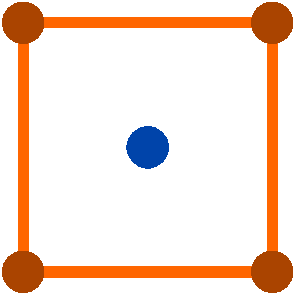
\includegraphics[scale=0.8]{chapter4-outilPoint4-pstricks}
  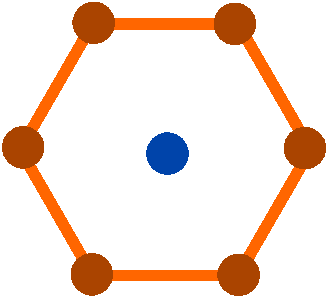
\includegraphics[scale=0.8]{chapter4-outilPoint6-pstricks}
  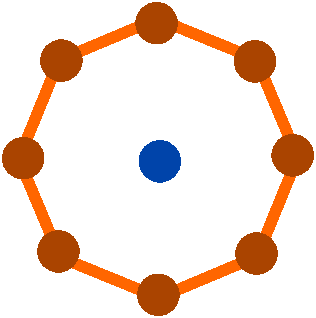
\includegraphics[scale=0.8]{chapter4-outilPoint8-pstricks}

  \caption[Cages d'influence à partir d'un point] {Différentes cages
d'influence créées à partir d'un point comme outil de contrôle.}
  \label{EXTPoi}

\end{center}
\end{figure}

Dans le même esprit, nous pourrions obtenir une cage d'influence à partir
d'une courbe. La cage d'influence serait générée comme un épaississement de la
courbe. Le lien entre la courbe et la cage d'influence pourrait se faire comme
pour les cages de contrôle. Mis à part qu'ici au lieu de modifier la position
d'un seul sommet, un point de contrôle modifierait la position des deux
sommets qui résultent de l'épaissement de la courbe au niveau de ce point de
contrôle (Figure \ref{EXTCou}).

\begin{figure}[ht]
\begin{center}
  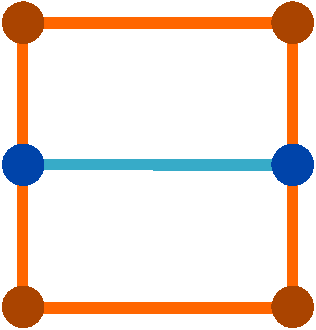
\includegraphics[scale=0.8]{chapter4-outilCourbe4-pstricks}
  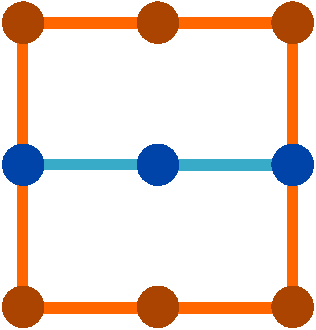
\includegraphics[scale=0.8]{chapter4-outilCourbe6-pstricks}
  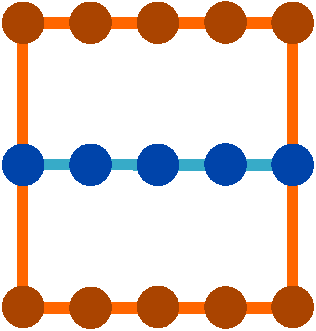
\includegraphics[scale=0.8]{chapter4-outilCourbe10-pstricks}

  \caption[Cages d'influence à partir d'une courbe] {Différentes cages
d'influence créées à partir de courbes de différentes résolutions comme outils
de contrôle.}

  \label{EXTCou}

\end{center}
\end{figure}

\section{Mélange d'outils existants}

Plusieurs outils existent déjà, comme nous avons pu le voir dans le chapitre
qui fait l'état de l'art des outils de déformation spatiale. On se demande
alors si notre technique permet le mélange de certains de ces outils. Et si
c'est possible, comment notre technique pourrait permettre de mélanger ces
différents outils ensemble.

Un point important de la méthode de mélange proposée dans ce travail est la
notion de \textit{distance à l'outil}. En effet, c'est grâce à cette distance
que l'importance de l'atténuation peut être évaluée. A partir du moment où un
outil permet de connaître la position d'un point de l'espace par rapport à la
position des points de contrôle de cet outil et au bord du domaine
d'influence, la technique de mélange présentée au chapitre précédent devrait
fonctionner.

Il est évident que les outils de déformation dont l'influence est globale ne
peuvent pas être utilisés tels quels, car ils n'ont pas un domaine d'influence
fini. Néanmoins, comme nous l'avons fait pour les déformations à base de
cages, il devrait être possible de rendre leur influence locale. Une fois le
domaine d'influence défini, il serait possible d'évaluer le critère de
"distance à l'outil". Cette distance calculée nous permettrait dans un premier
temps de modifier partiellement un modèle grâce à un outil de déformation,
mais aussi de mélanger plusieurs outils ensembles (à condition que chacun
puisse définir cette notion de distance).

Ces réflexions sont purement théoriques et certaines suppositions pourraient
être fausses, néanmoins nous pensons que des réflexions plus poussées dans ces
directions seraient intéressantes pour les travaux futurs.


\def\baselinestretch{1}
\chapter{My Conclusions ...}
\ifpdf
    \graphicspath{{Conclusions/ConclusionsFigs/PNG/}{Conclusions/ConclusionsFigs/PDF/}{Conclusions/ConclusionsFigs/}}
\else
    \graphicspath{{Conclusions/ConclusionsFigs/EPS/}{Conclusions/ConclusionsFigs/}}
\fi

\def\baselinestretch{1.66}

Here I put my conclusions ...

%%% ----------------------------------------------------------------------

% ------------------------------------------------------------------------

%%% Local Variables: 
%%% mode: latex
%%% TeX-master: "../thesis"
%%% End: 


\appendix

\chapter{Appdx A}

and here I put a bit of postamble ...

% ------------------------------------------------------------------------

%%% Local Variables: 
%%% mode: latex
%%% TeX-master: "../thesis"
%%% End: 

% \include{Appendix2/appendix2}

\bibliographystyle{plainnat}
%\bibliographystyle{Classes/CUEDbiblio}
% \bibliographystyle{Classes/jmb}
% \bibliographystyle{Classes/jmb} % bibliography style
\renewcommand{\bibname}{Références} % changes default name Bibliography to References
\bibliography{References/references} % References file

\end{document}